    \section{Motivation}
    Um die Einflüsse verschiedener Kurzschlussanordnungen und -ausführungen schon im Vorfeld abschätzen zu können und ein erstes Gefühl für den Einfluss der Kurzschlüsse zu bekommen, wurde die Testanordnung zunächst ausgiebig mit der Simulationssoftware CST simuliert.\\
    Die Simulationen dienten als Vorbereitung, um bei den Messungen präziser vorgehen zu können und gezielt Messungen durchzuführen. Zuletzt wurden die Simulationsergebnisse dann mit den Messergebnissen gegenübergestellt und verglichen, um deren Richtigkeit zu überprüfen.
    
    \section{Modellierung}
        \subsection{Bestehendes Testbox- und Ringkernmodell}
        Als Grundlage für die Simulation der Testbox und des Ringkerns dient das Simulationsmodell von Testbox inklusive Ringkern aus der Bachelorarbeit von Denys Bast \citep{bast2017ba}.\\
        Die Außenwände der Testbox sind geometrisch sehr genau den Abmessungen des realen Teststandes entsprechend modelliert, als Material wird hierfür reines Kupfer verwendet, wie es in der Datenbank von CST zu finden ist. Die leere Box ist in Abbildung~\ref{fig:BoxCST} dargestellt.
        
            \begin{figure}[htb]
                \centering
                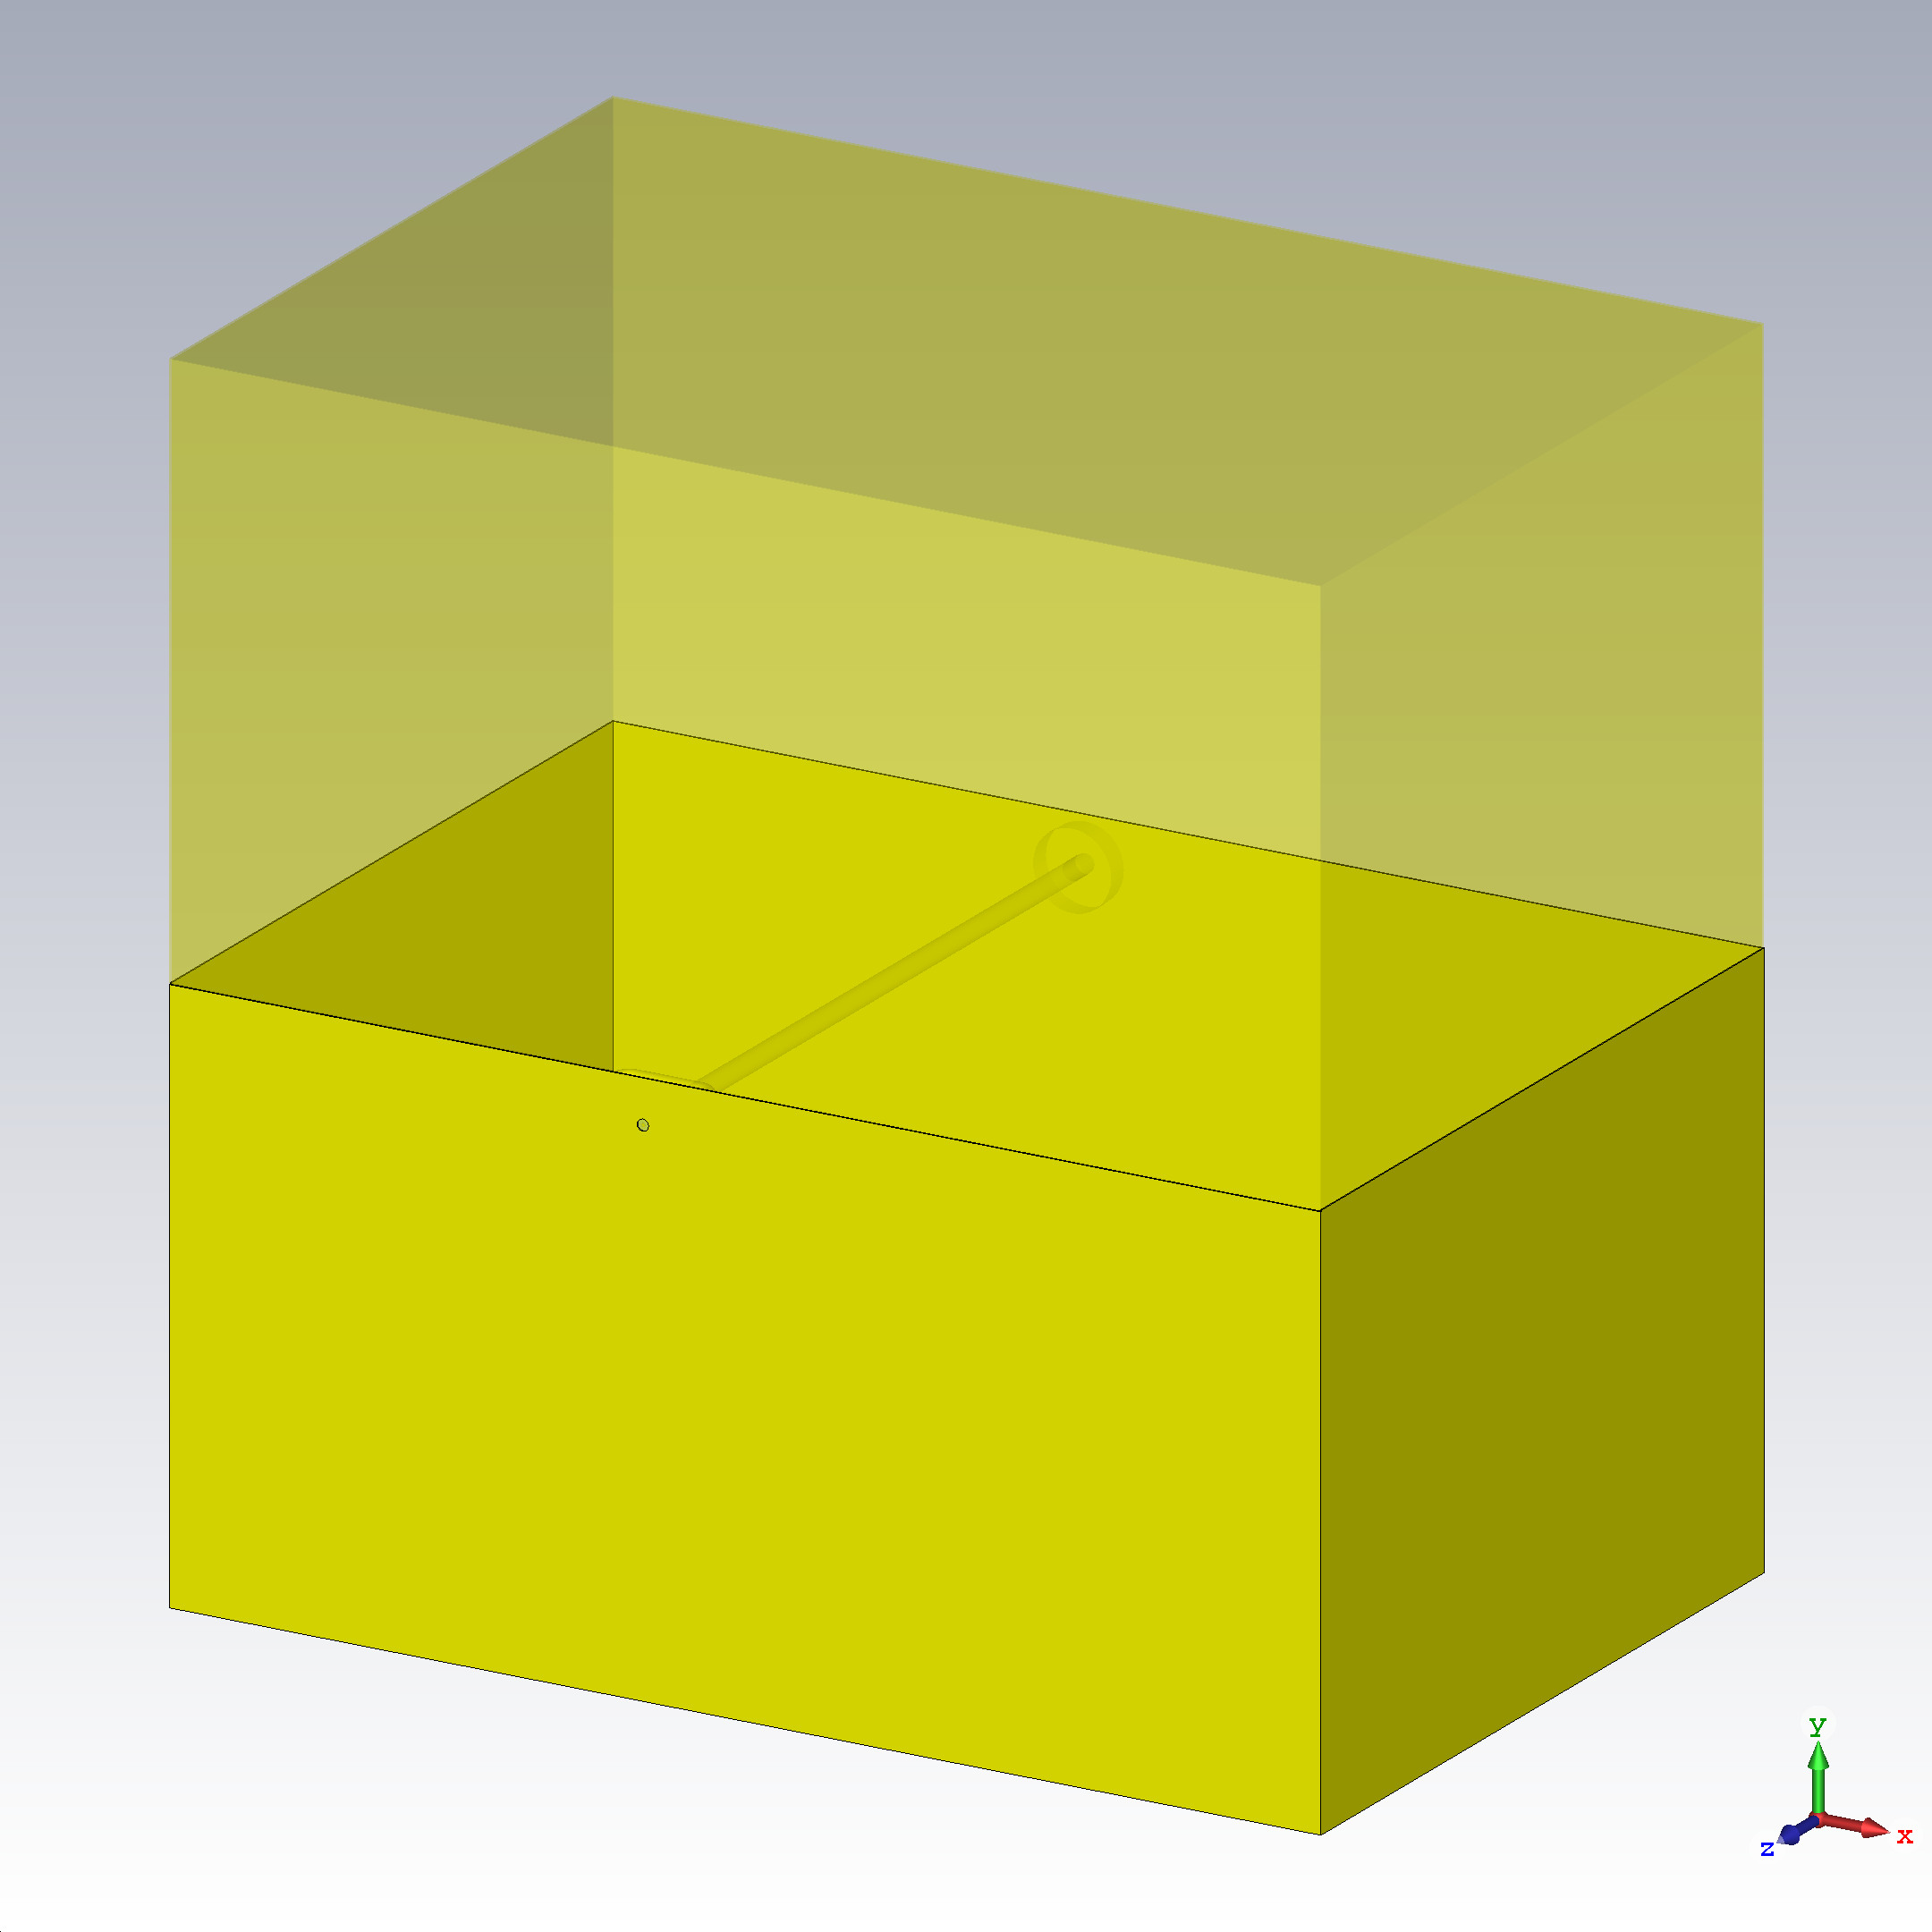
\includegraphics[height=0.4\textwidth]{./Simulation/BoxWaende2.png}
                \caption{Modell der Testbox in CST}
                \label{fig:BoxCST}
            \end{figure}
        In Abbildung~\ref{fig:InnenleiterCST} ist die Signaleinkopplung der Testbox zu sehen.
        Diese ist als Hohlzylinder aus Kupfer modelliert und geometrisch genau am realen Vorbild orientiert. Die Stange ist an der hinteren Wand elektrisch mit der Box verbunden und an der Vorderseite durch einen elektrisch nicht leitfähigen Ring aus Polyethylen (PE, CST Datenbank) von der Box isoliert. Hierdurch wird erreicht, dass die Stange als Hin- und die Boxaußenwände als Rückleiter für Signale dienen. Der Übergang zwischen Testbox, PE und Stange ist planar ausgeführt, um einen Signalport für die Simulation darzustellen.
        
            \begin{figure}[htb]
                \centering
                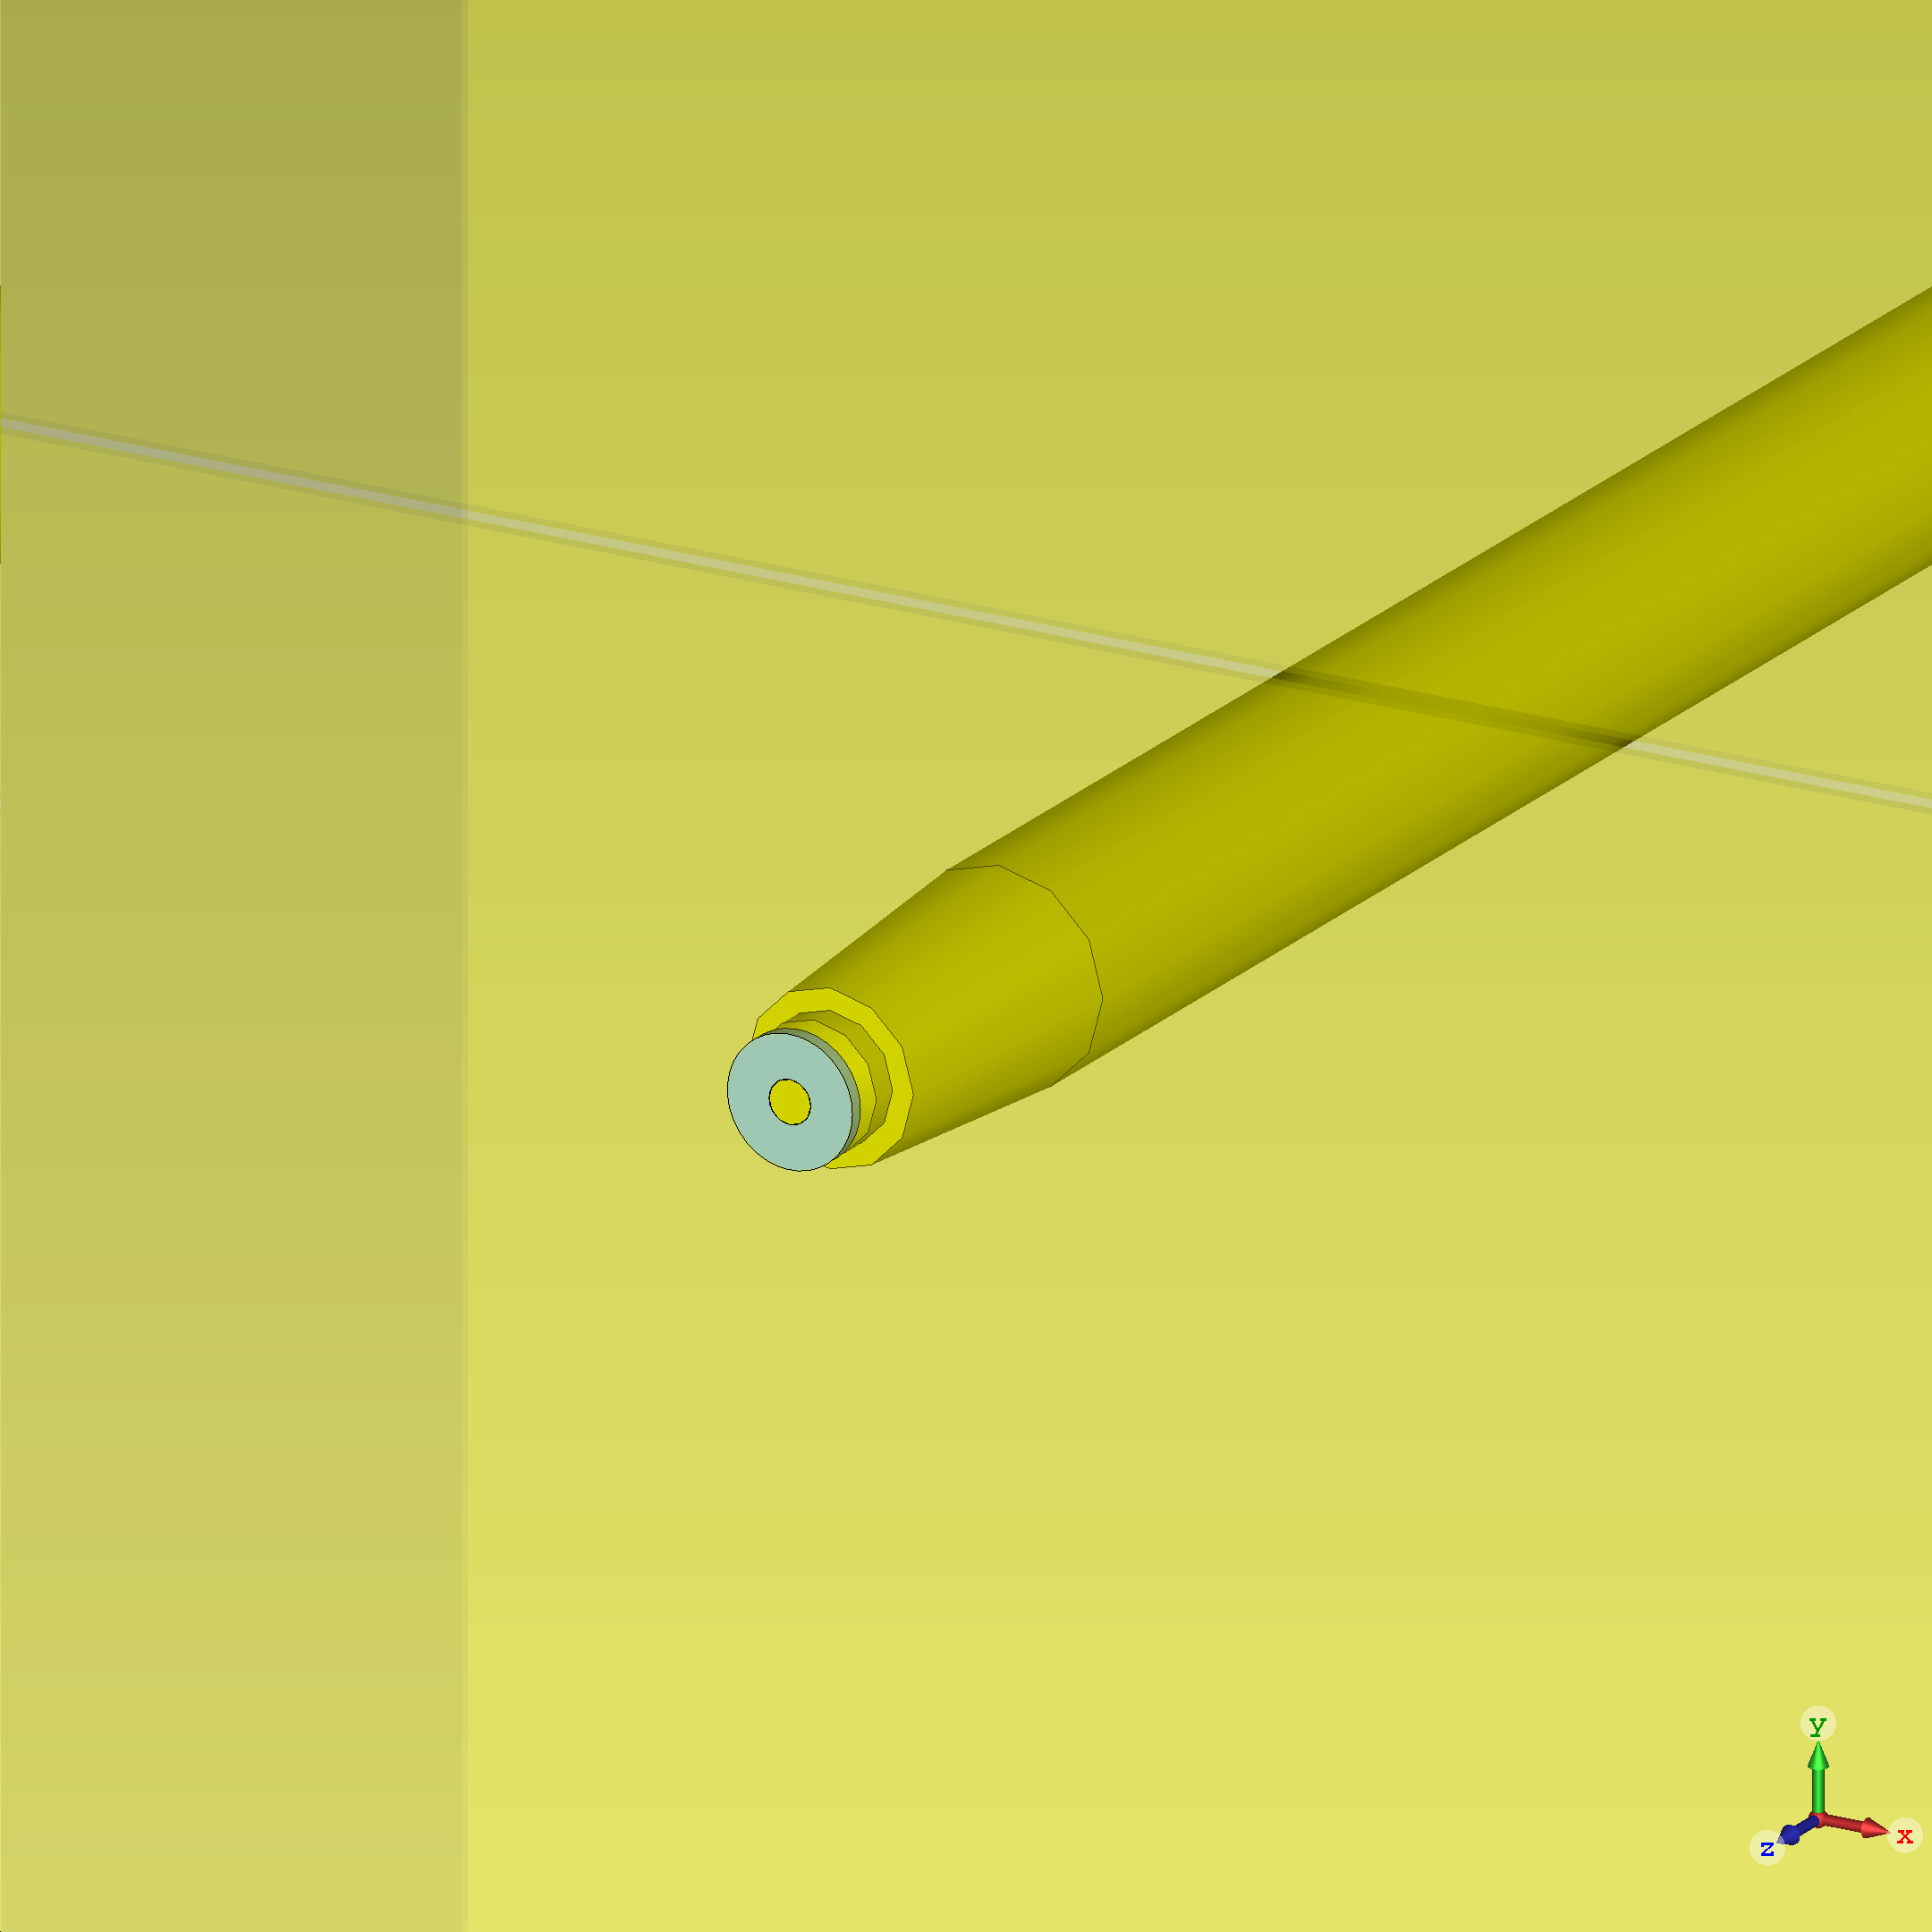
\includegraphics[height=0.4\textwidth]{./Simulation/InnenleiterPE.png}
                \caption{Modell der Einkopplungsstange mit elektrischer Isolation}
                \label{fig:InnenleiterCST}
            \end{figure}
        
        Der Ringkern ist als einfacher Hohlzylinder mit den geometrischen Abmessungen seines realen Vorbild modelliert. Dem realen Aufbau entsprechend ist er zentral im Testboxmodell, allerdings freischwebend, ohne die hölzerne Halterung, modelliert.\\
        Ein grundlegender Aspekt der Arbeit von Denys Bast~\citep{bast2017ba} ist, die magnetische Permeabilität des Ringkernmaterials in der Simulation mit dem realen Material in Übereinstimmung zu bringen. Die dabei gewonnenen Daten wurden übernommen.
        
            \begin{figure}[htb]
                \centering
                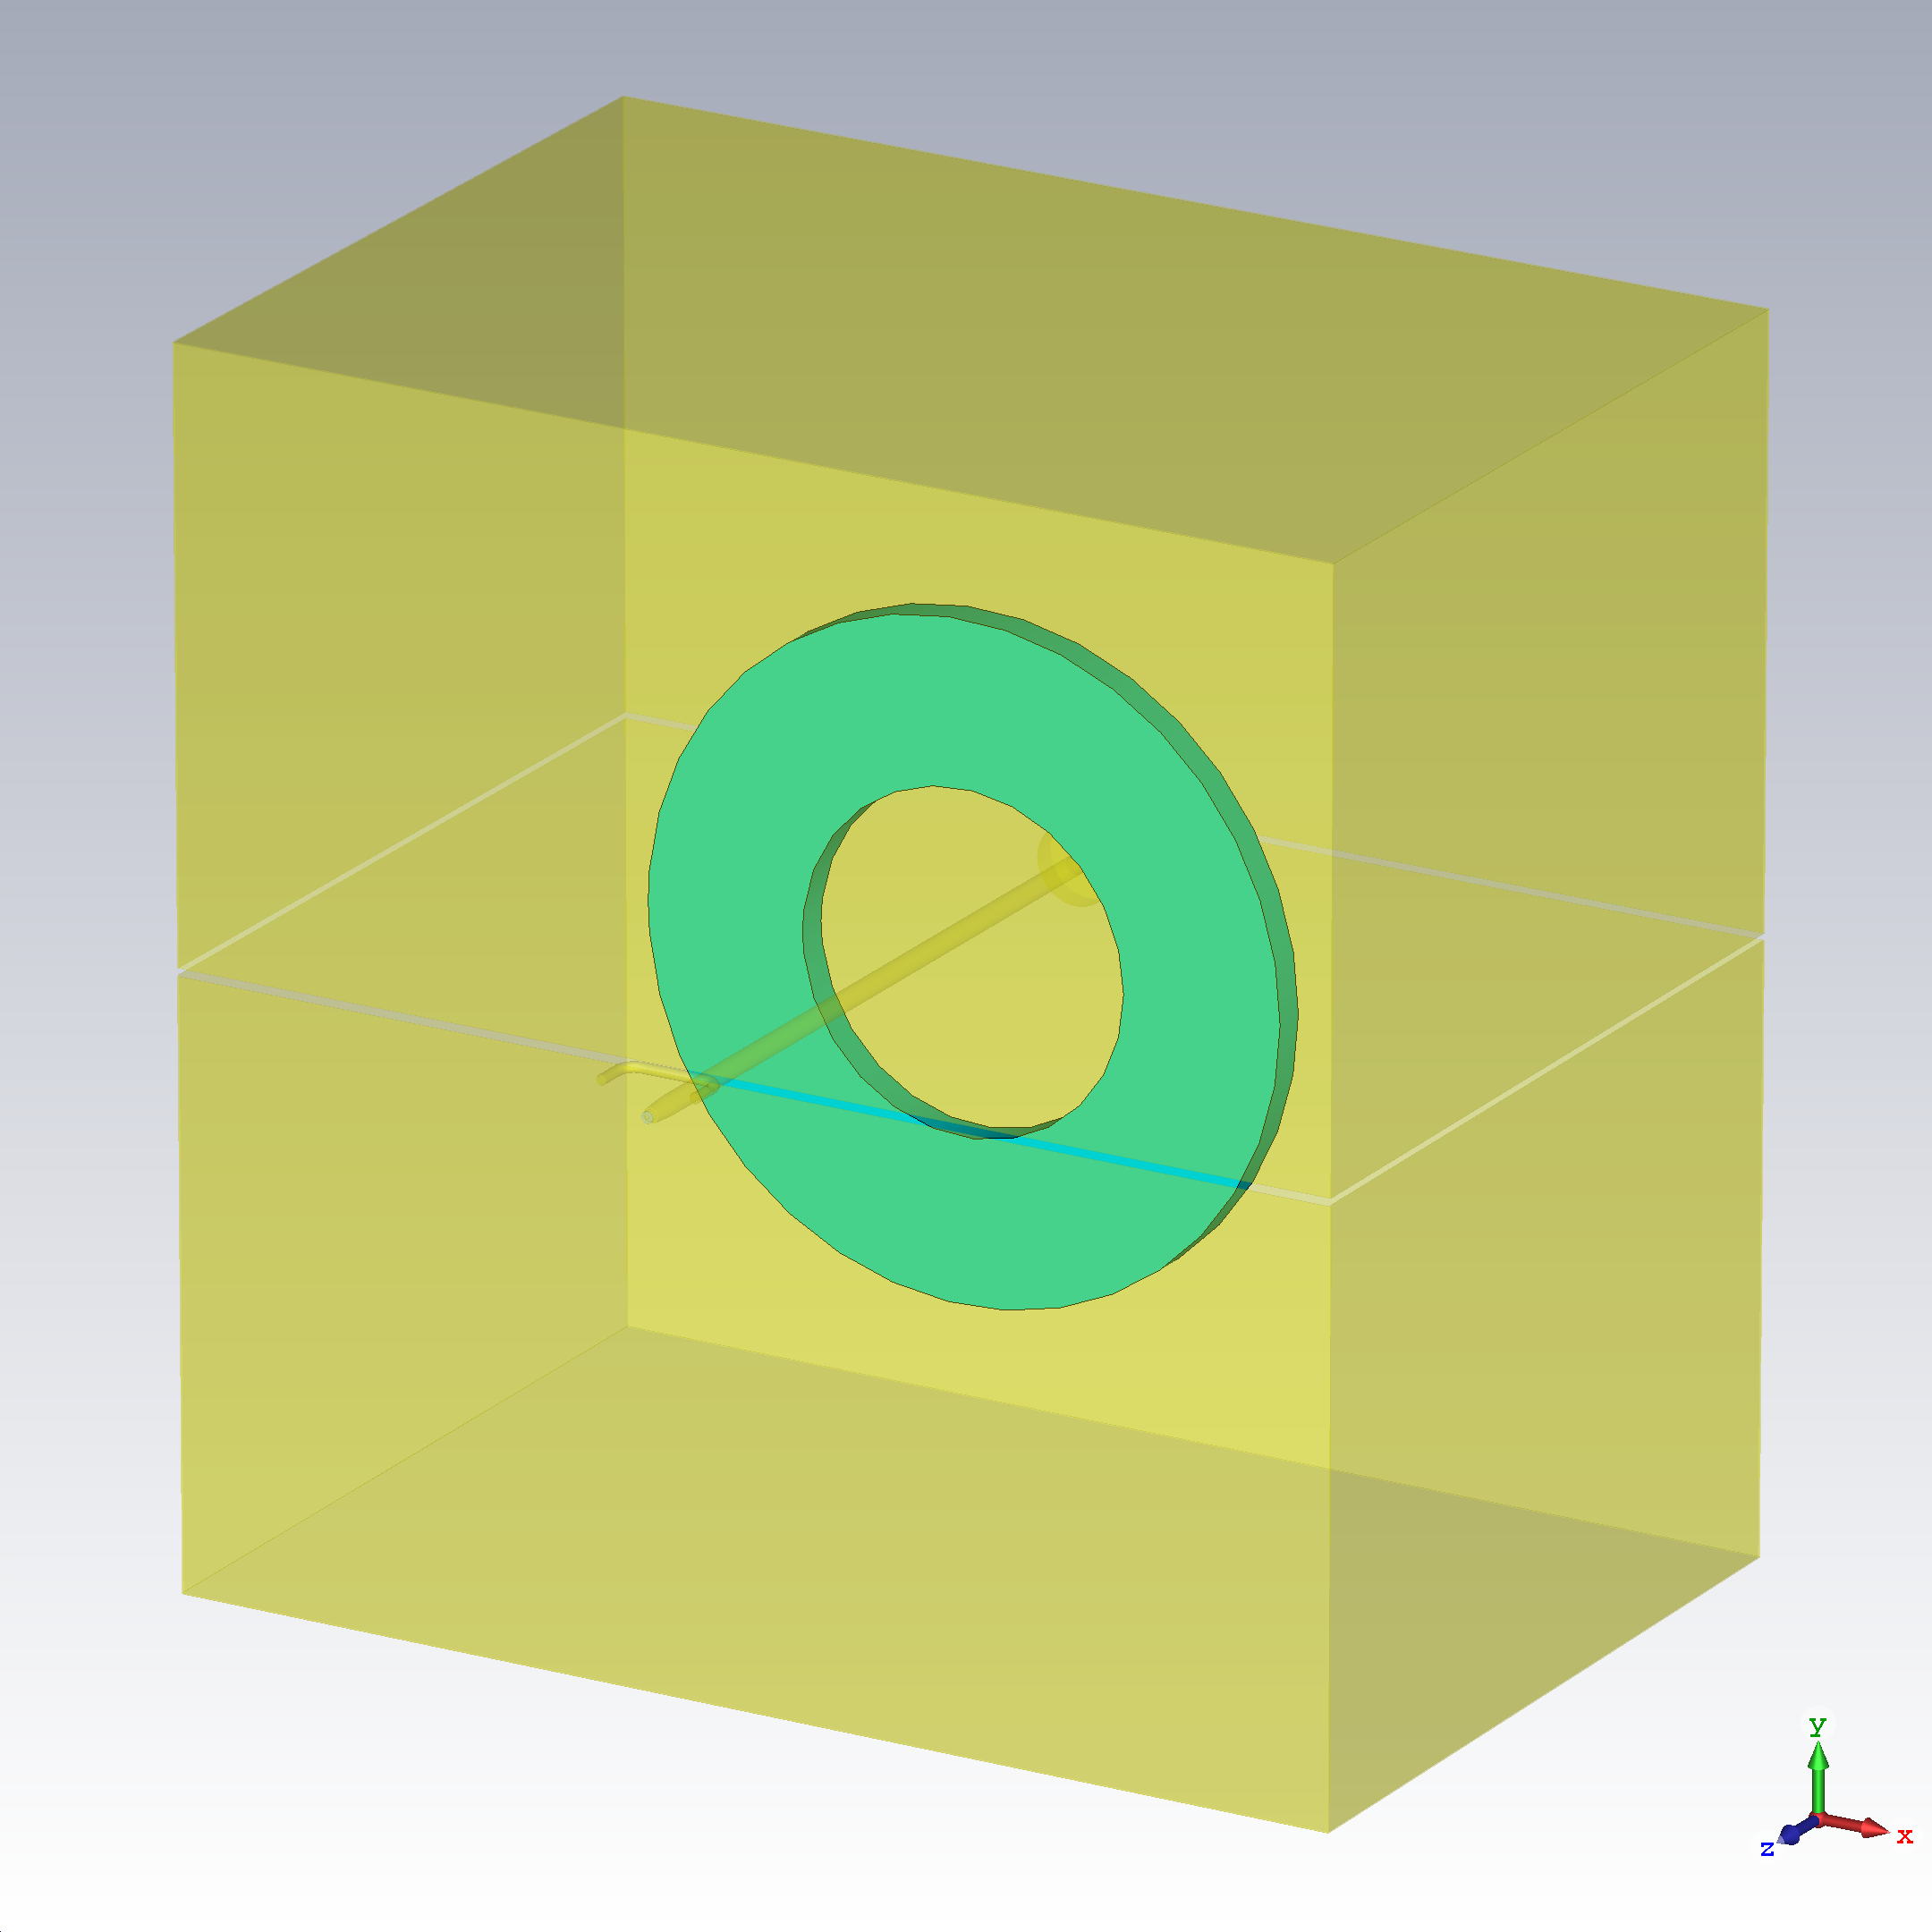
\includegraphics[height=0.4\textwidth]{./Simulation/BoxRK.png}
                \caption{Gesamtdarstellung der Modellierung von Testbox und Ringkern nach Denys Bast~\citep{bast2017ba}}
                \label{fig:BoxRKCST}
            \end{figure}
        
        Abbildung~\ref{fig:BoxRKCST} bildet den modellierten Aufbau der Testbox mit Ringkern ab, wie er in \citep{bast2017ba} beschrieben wird.

        \subsection{Kurzschlüsse}
        Die für die Parameteranalyse dieser Arbeit benötigten Kurzschlüsse sind in CST in verschiedenen, komplexen Ausführungen modelliert.\\
        Die erste Version stellt ein einfacher, ellipsenförmiger Torus dar, wie er in Abbildung~\ref{fig:KSCST}\subref{subfig:V1} abgebildet ist. Als Material für die Simulation wird Kupfer aus der Datenbank von CST verwendet.\\
        Die in Kapitel~\ref{sec:testbox} beschriebenen Verbesserungen der Kurzschlüsse für eine erhöhte Reproduzierbarkeit der Messungen, sind so in CST modelliert. Abbildung~\ref{fig:KSCST}\subref{subfig:V2} zeigt die Umformung des einfachen Torus zu einem schienenförmigen Kurzschluss. Die finale Version, die letztlich für die Messungen benutzt wurde, ist in Abbildung~\ref{fig:KSCST}\subref{subfig:V3} zu sehen. Die einfache Kupferschiene ist geometrisch an die verwendeten Kurzschlüsse angepasst und um die Verbindungsschrauben erweitert.
        
            \begin{figure}[htb]
                \centering
                \subfloat[Version 1]{
                    \label{subfig:V1}
                    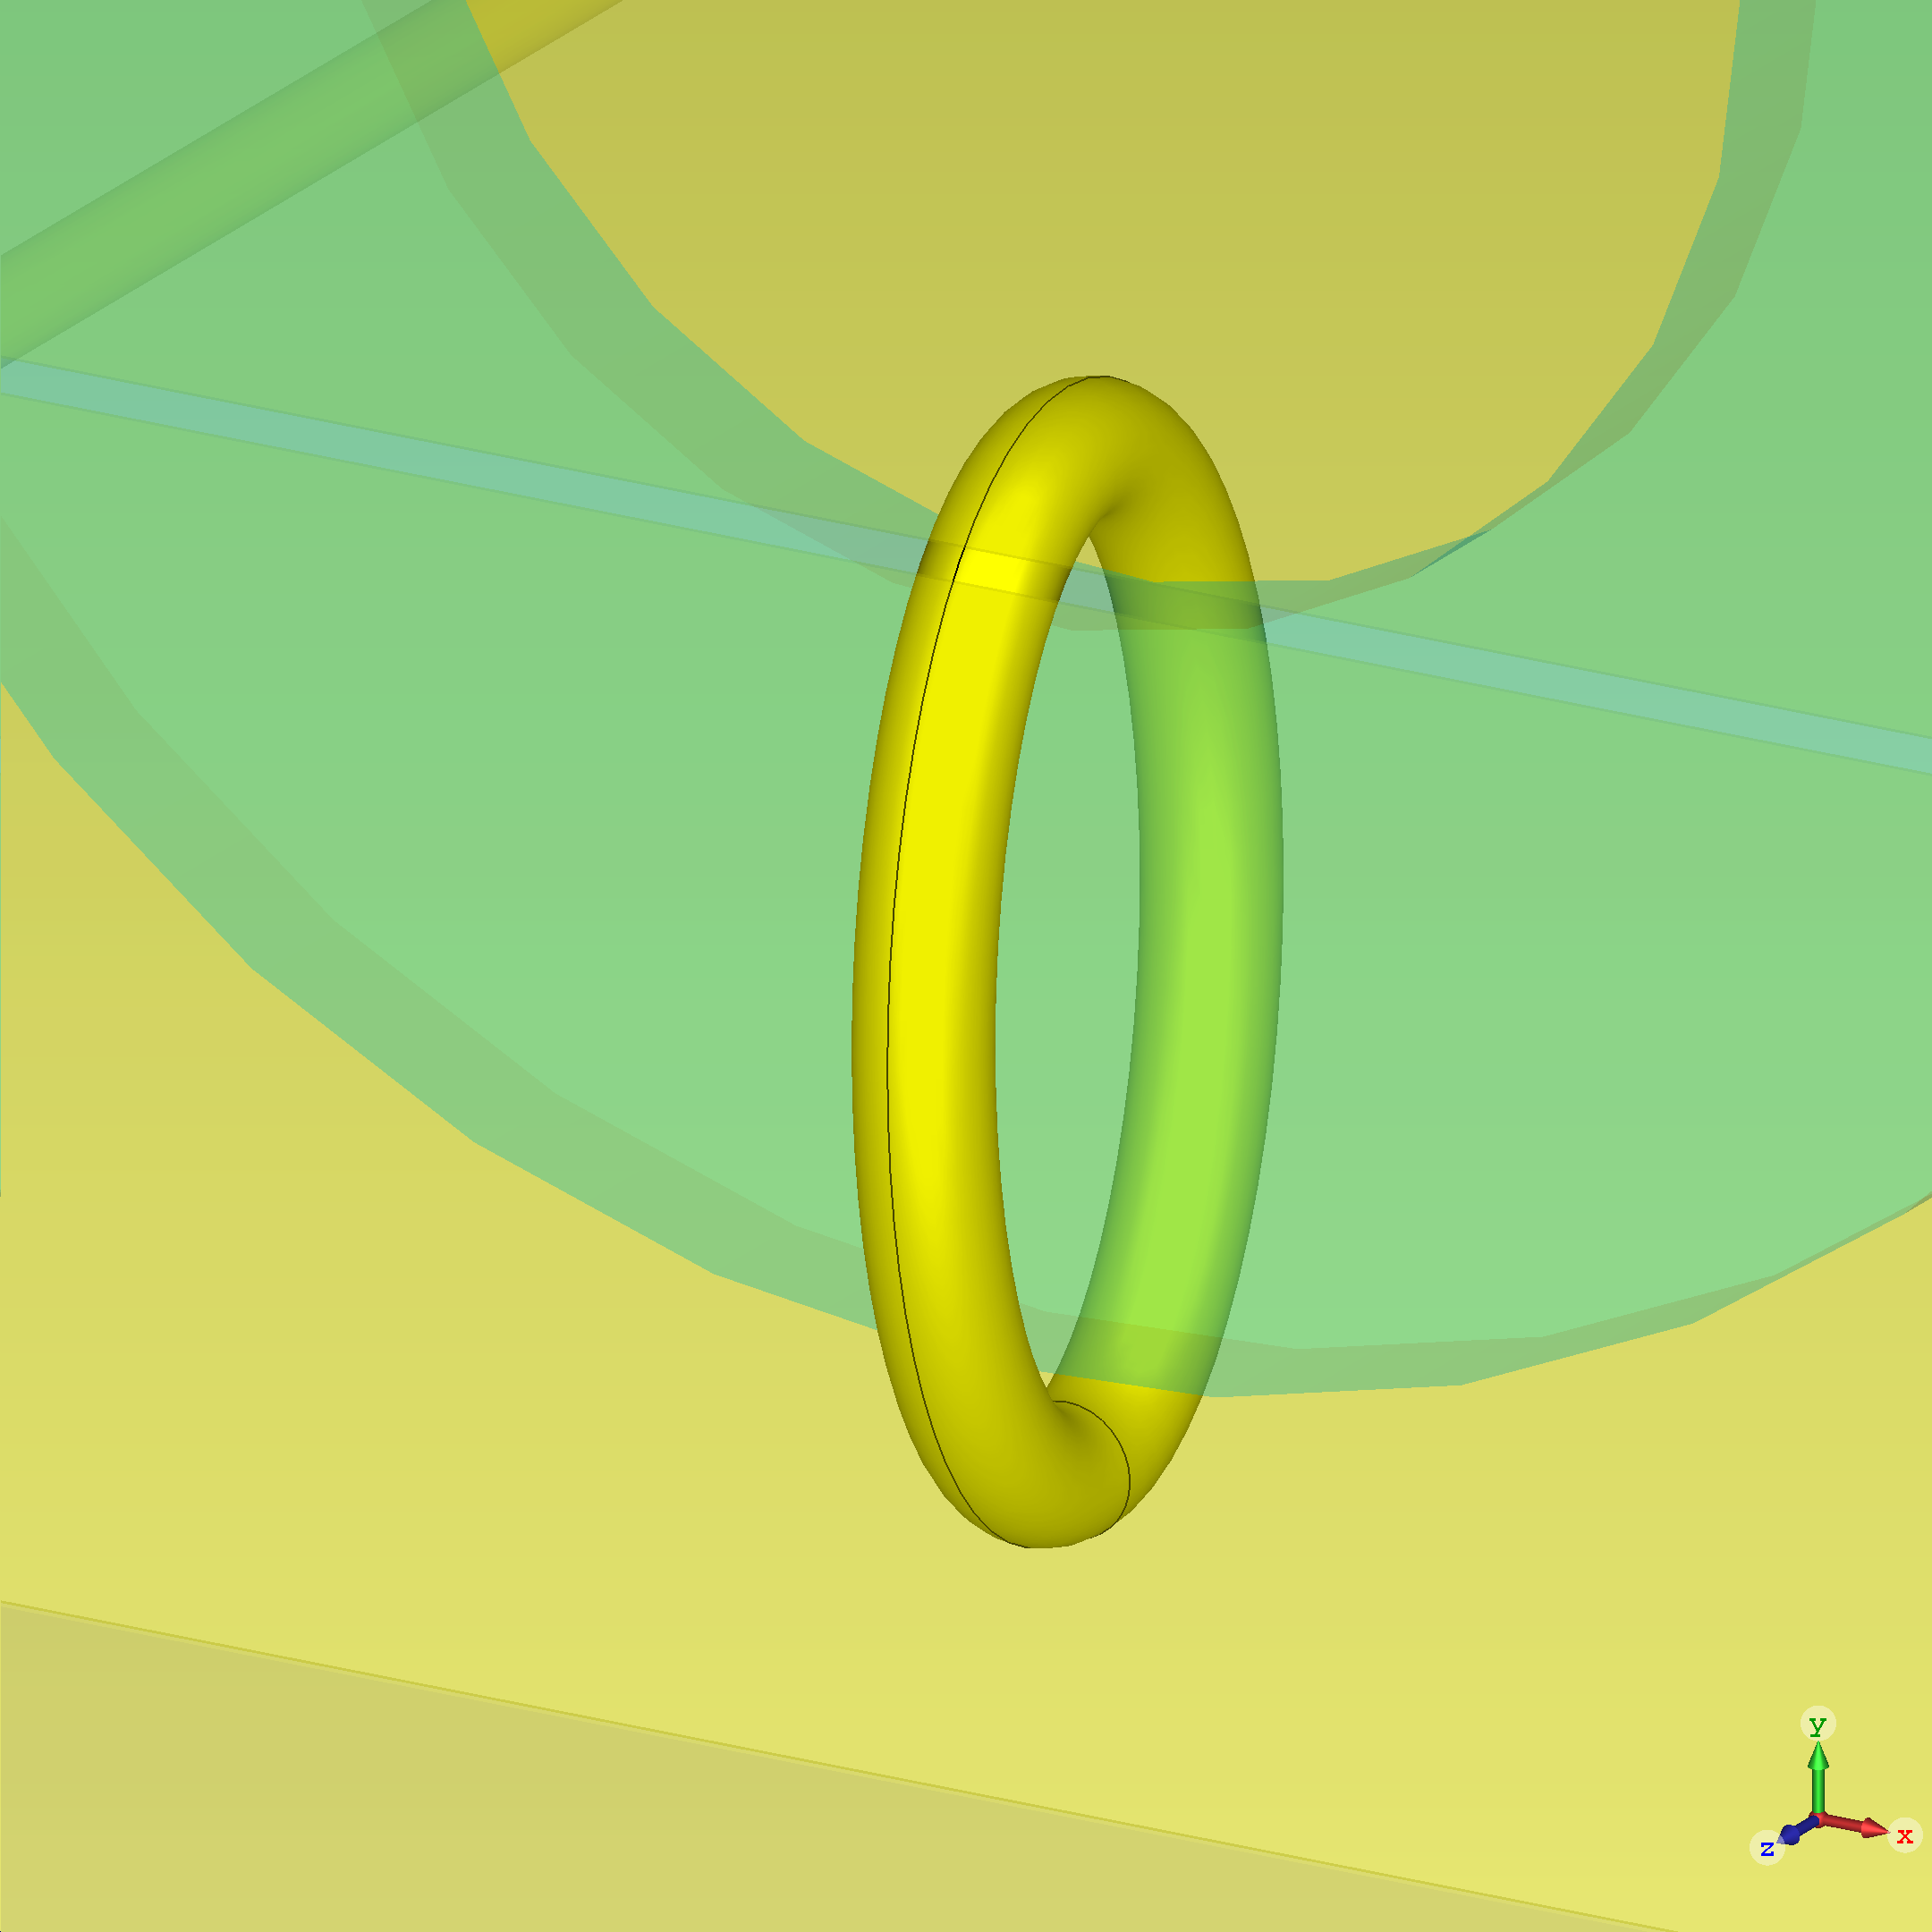
\includegraphics[height=0.3\textwidth]{./Simulation/KSV1Torus.png}}
                \hspace{0.01\textwidth}
                \subfloat[Version 2]{
                    \label{subfig:V2}
                    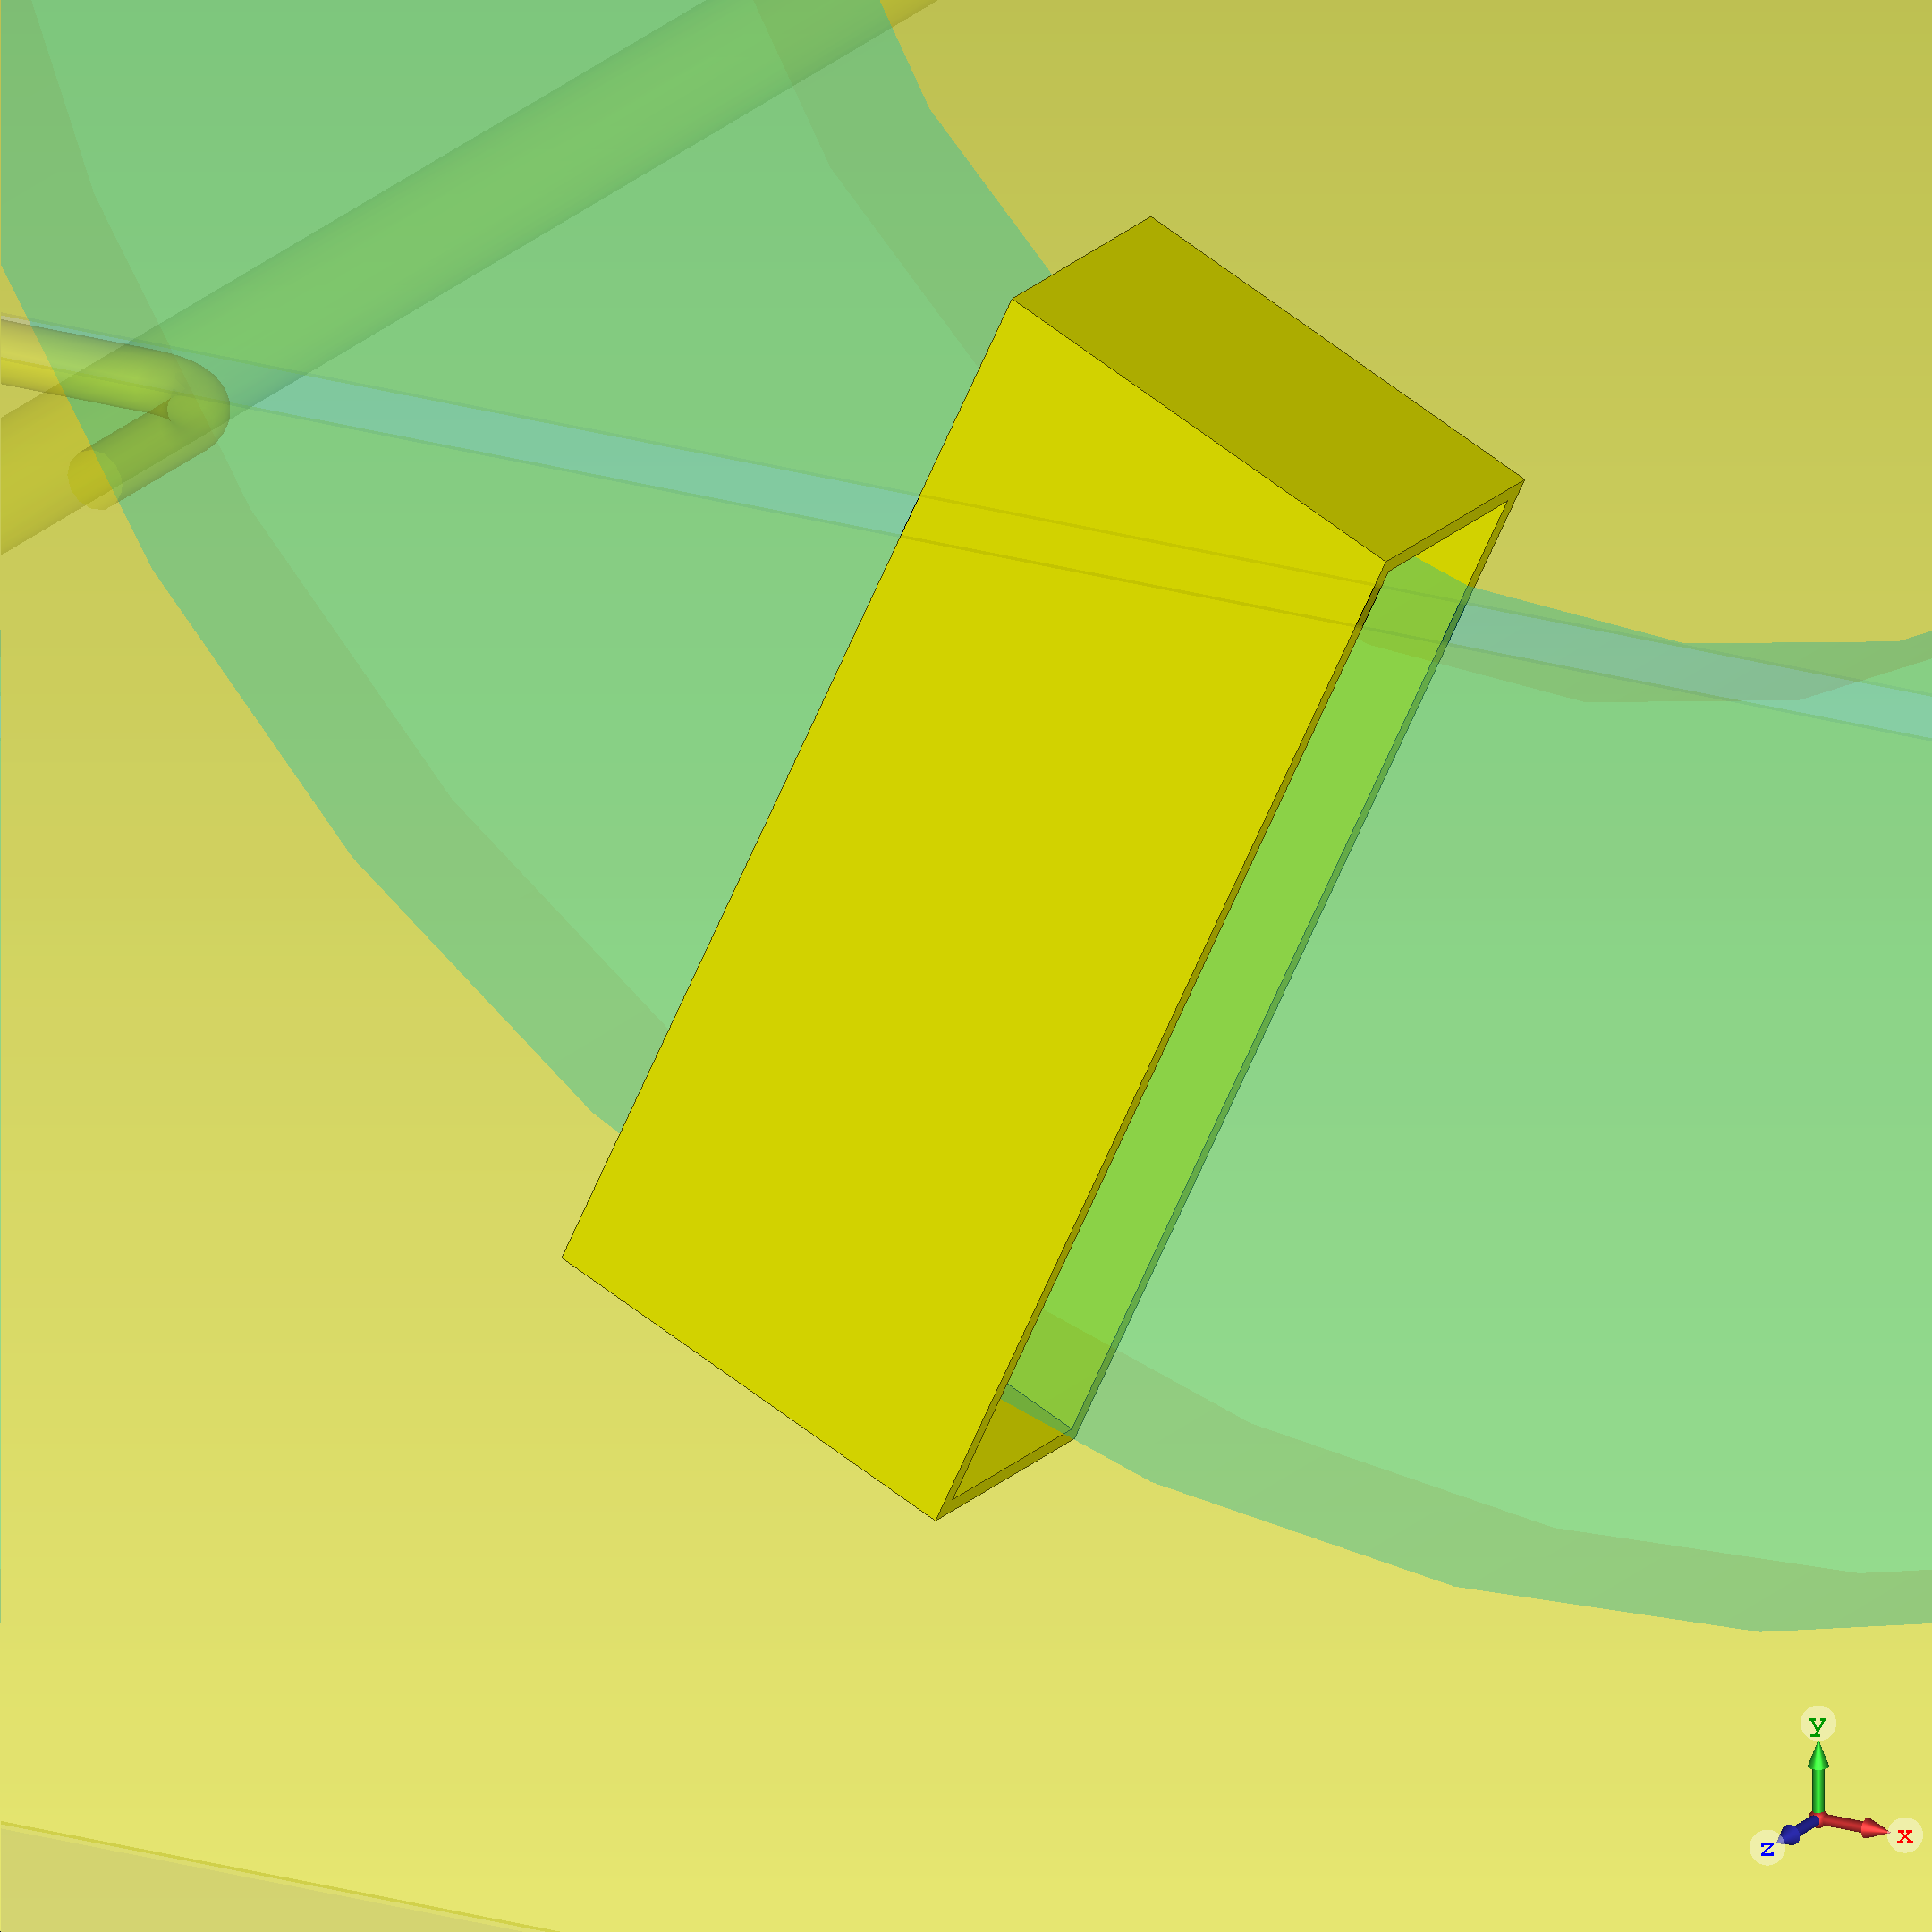
\includegraphics[height=0.3\textwidth]{./Simulation/KSV2Schiene.png}}
                \hspace{0.01\textwidth}
                \subfloat[Version 3]{
                    \label{subfig:V3}
                    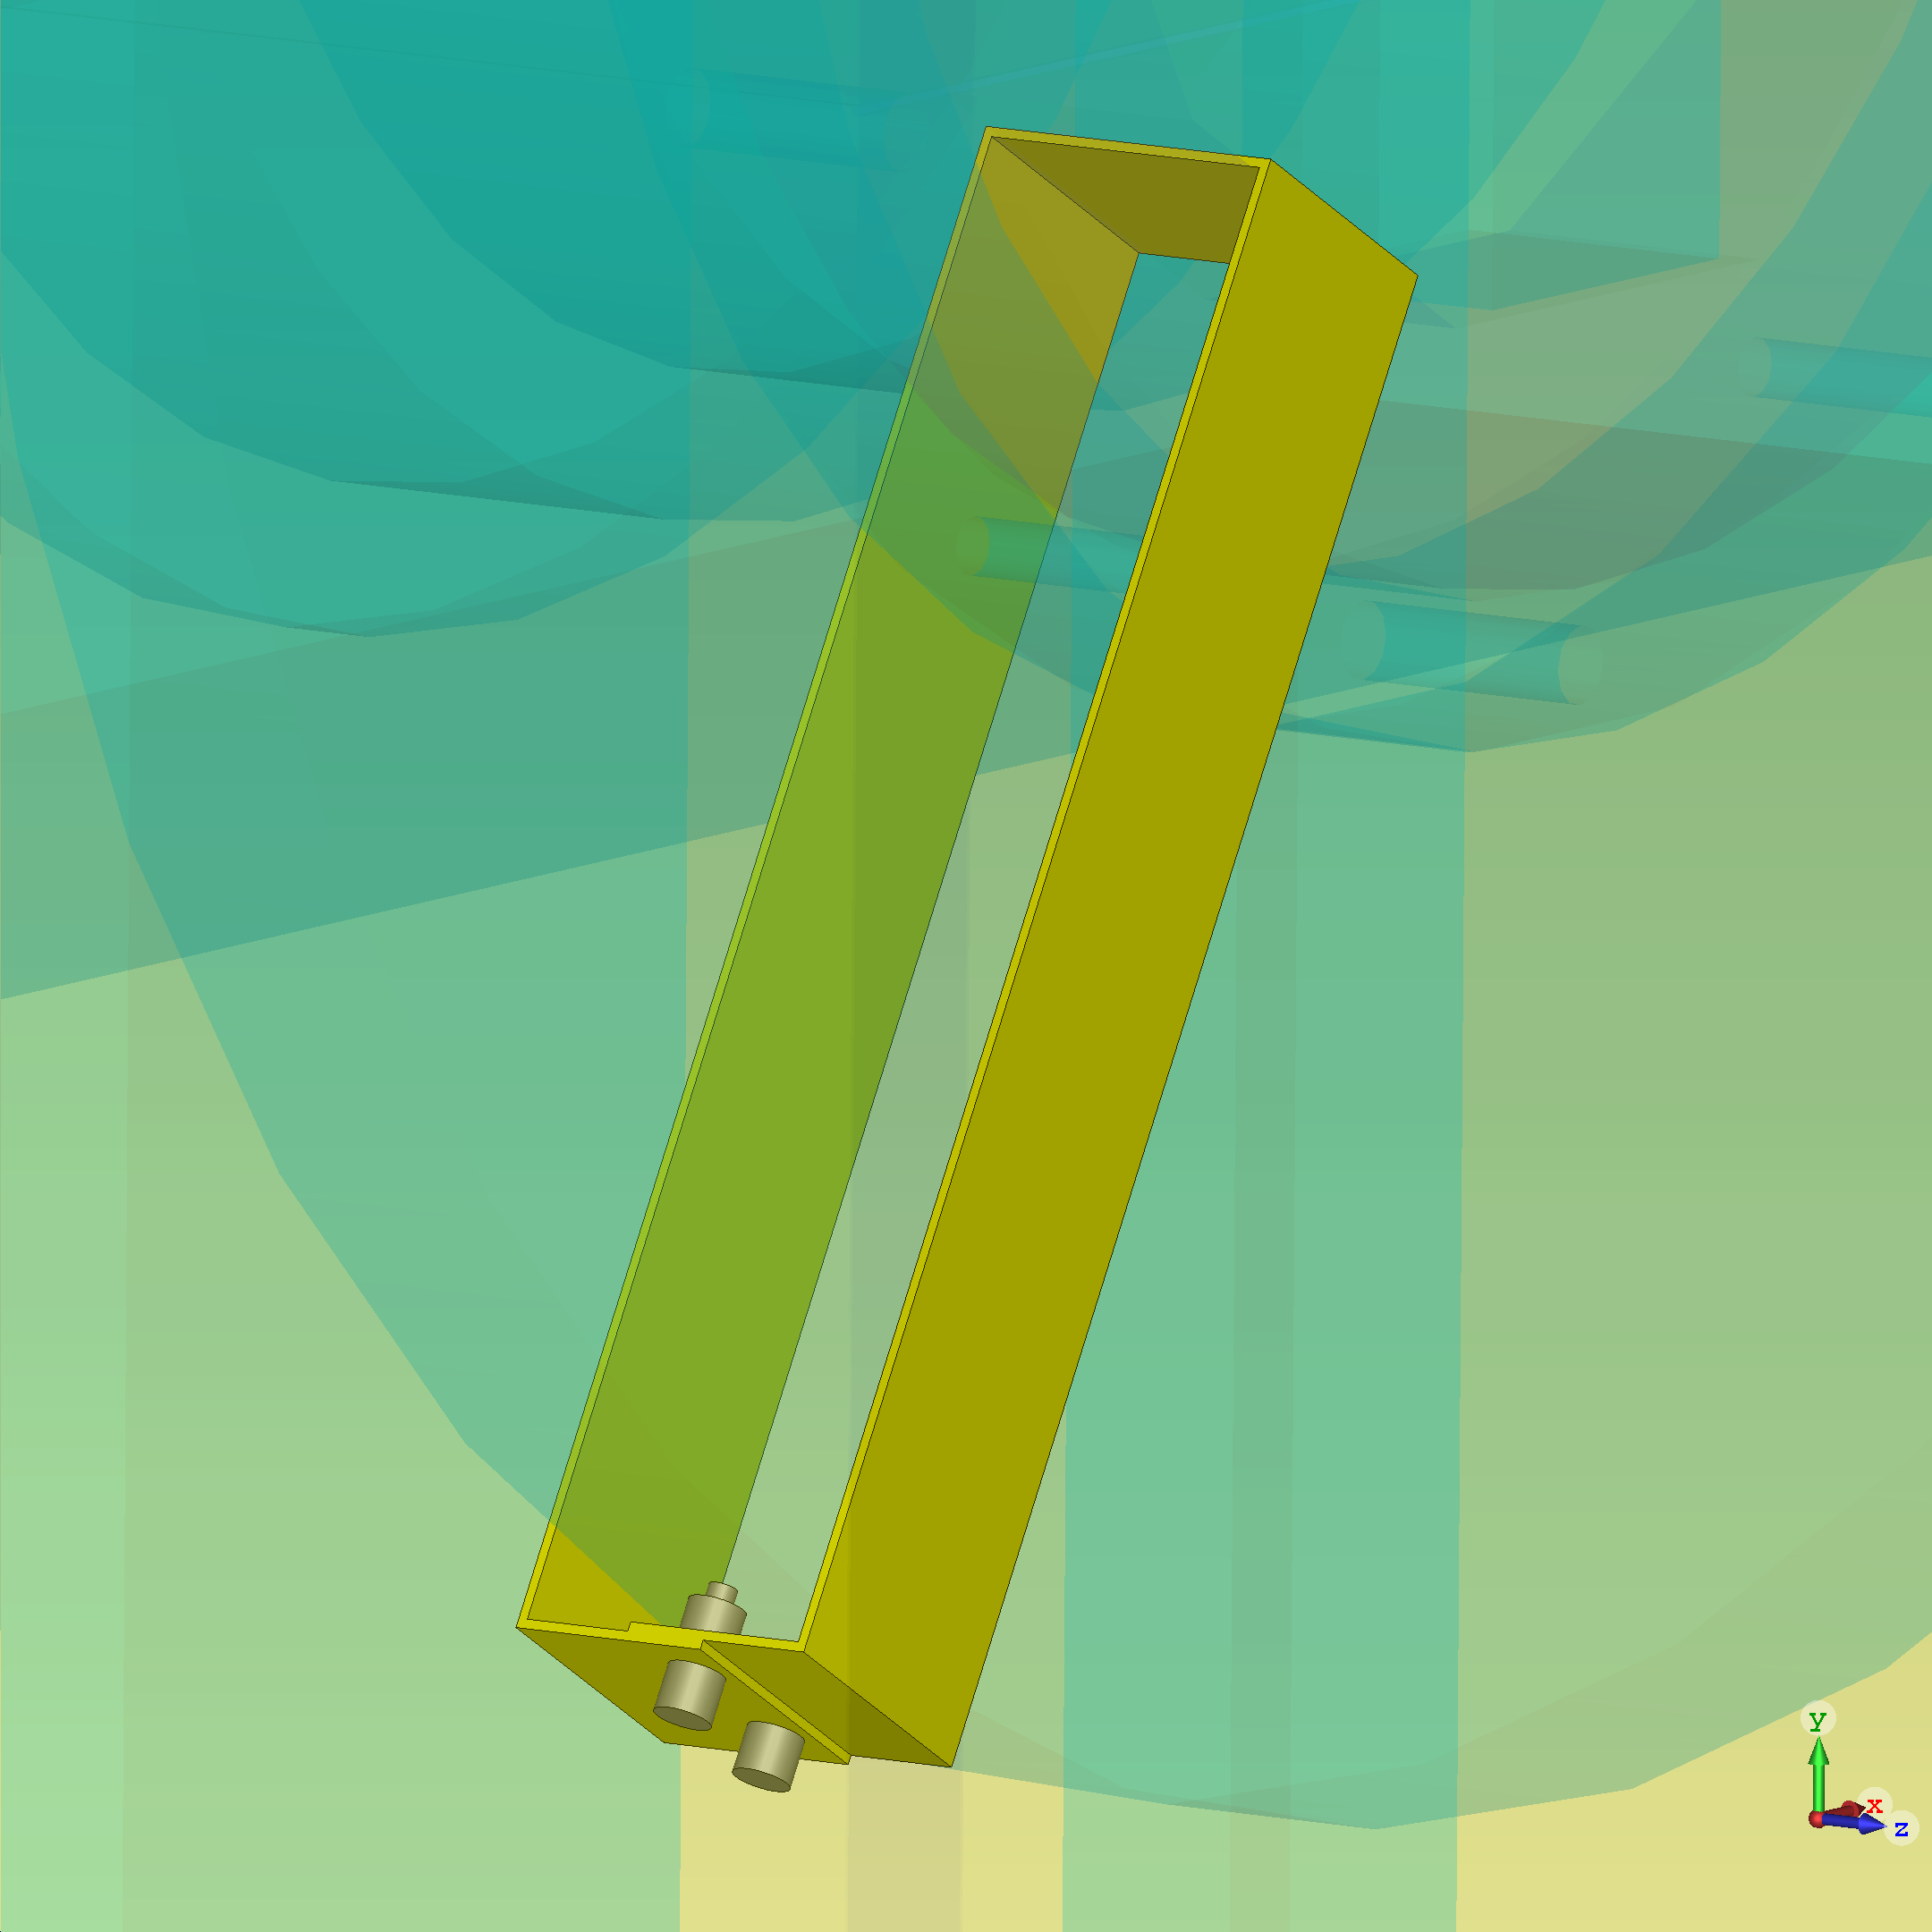
\includegraphics[height=0.3\textwidth]{./Simulation/KSV3MitSchrauben.png}}
                \caption{Modellierung eines Kurzschluss \protect\subref{subfig:V1} als Torus, \protect\subref{subfig:V2} als Schiene und \protect\subref{subfig:V3} in gefertigter Ausführung.}
                \label{fig:KSCST}
            \end{figure}
        
        Um eine Parameteranalyse durchzuführen und die Simulationsergebnisse mit den Messungen gegenüberzustellen, ist die finale Version in den verschiedenen Ausführungen, wie sie aus Kapitel~\ref{sec:shorts} hervorgehen, nachgebildet.
        
        \subsection{Realitätsgetreue Anpassungen}
        Das bestehende Modell wurde im Laufe der Arbeit weiter ausarbeitet, um die Übereinstimmung der Simulationsergebnisse mit den Messungen zu erhöhen. Die nachfolgenden Komponenten wurden in das CST-Modell übernommen, da aufgrund ihrer di-/elektrischen Eigenschaften ein Einfluss auf die Simulation zu erwarten ist.\\
        \todo[inline,color=red!30]{$\uparrow$ Verweis auf Simulationsergebnisse, wenn Kapitel vorhanden. $\uparrow$}
        Wie auf den Bildern der Testbox in Kapitel~\ref{chap:messaufbau} hervorgeht, befindet sich oberhalb der Einkopplungsstange an der Anschlussseite ein metallischer Bügel. Er ist möglichst exakt in CST nachgebildet (siehe Abb.~\ref{fig:AnpassungCST}\subref{subfig:Buegel}).\\
        Am Ende der Einkopplungsstange an der Rückwand ist eine zylinderförmige, kupferne Halterung für die Stange montiert, sie ist nach Abbildung~\ref{fig:AnpassungCST}\subref{subfig:Block} modelliert.
        \par
        Zuletzt wurde für diese Arbeit auch die Holzkonstruktion in CST übernommen, die als Halterung für die Ringkerne in der Testbox dient (siehe Abb.~\ref{fig:AnpassungCST}\subref{subfig:HolzKonst}). Dabei wurden die Holzkreise mit einem dissipativen, durch Austesten und die Messung Anpassen bestimmten $\underline{\varepsilon}_r(\omega) = \varepsilon_r'(\omega)-i\varepsilon_r''(\omega)$ modelliert, da es sich hierbei nicht um die Standardholzmodellierung von CST handelt, wie sie für die Holzbalken verwendet wird, sondern ein geschichtetes Pressspanholz verwendet wird.
        
            \begin{figure}[htb]
                \centering
                \subfloat[Bügel]{
                    \label{subfig:Buegel}
                    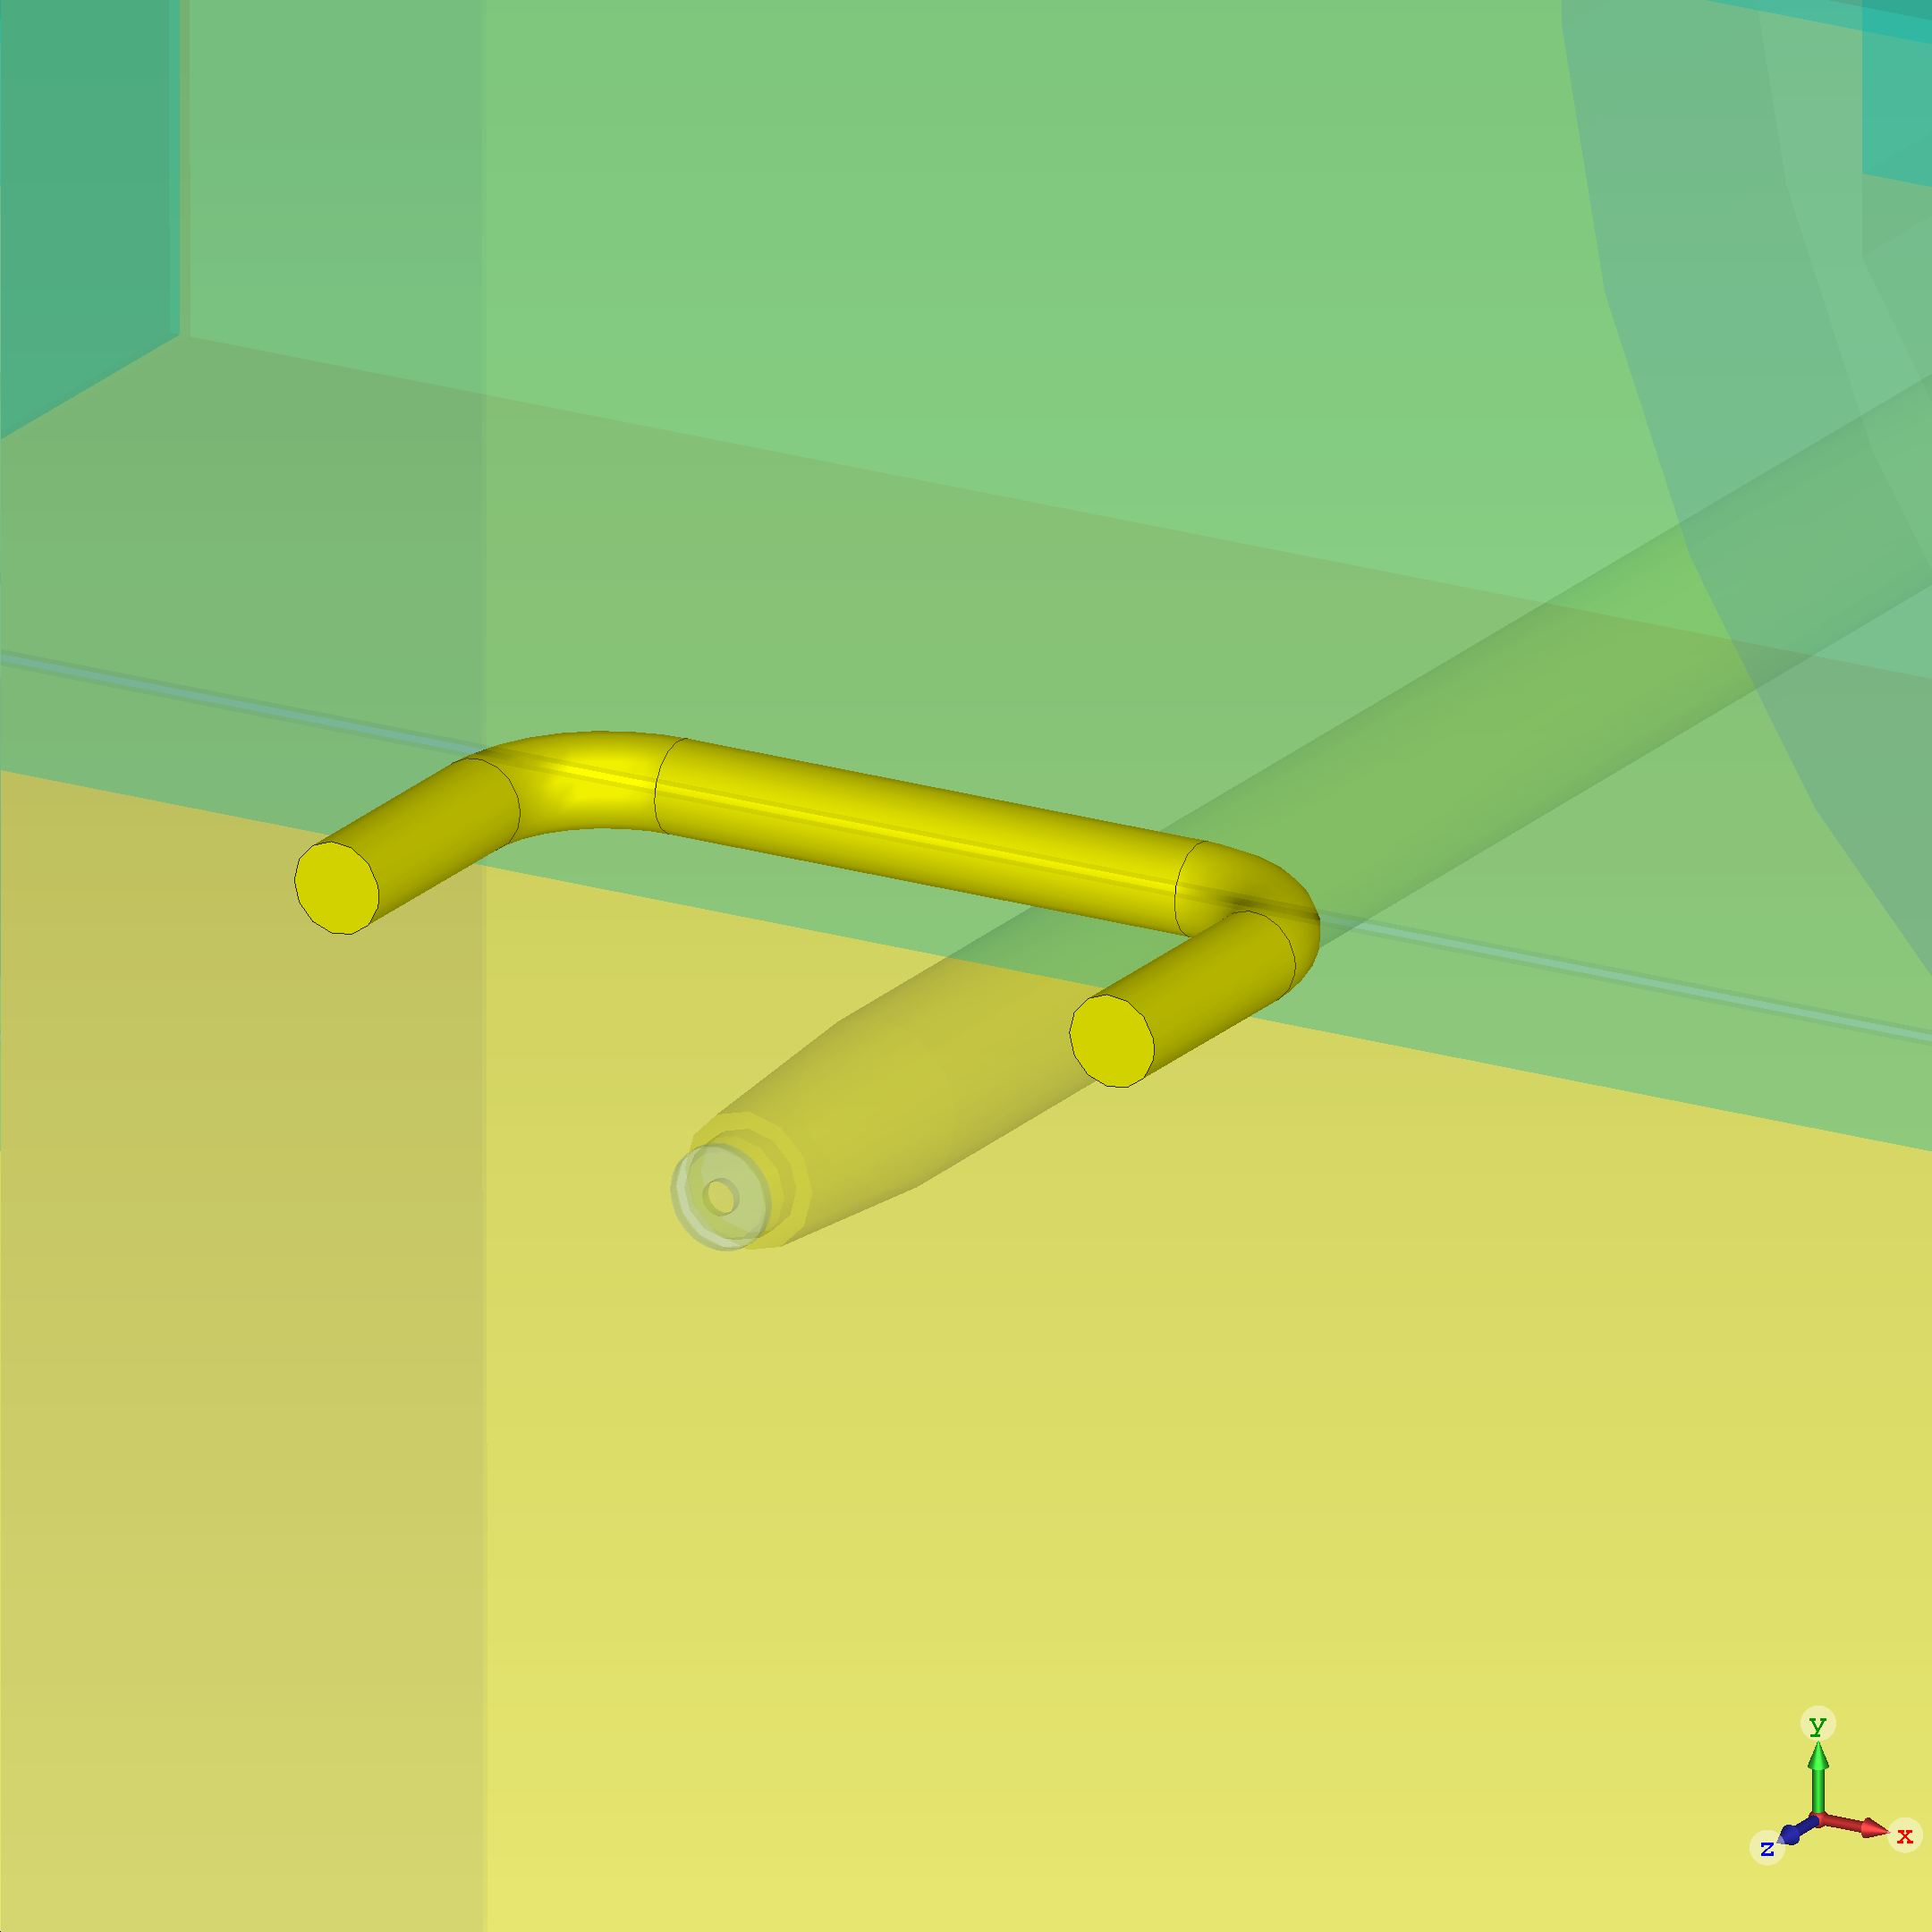
\includegraphics[height=0.3\textwidth]{./Simulation/Buegel.png}}
                \hspace{0.01\textwidth}
                \subfloat[Zylinder]{
                    \label{subfig:Block}
                    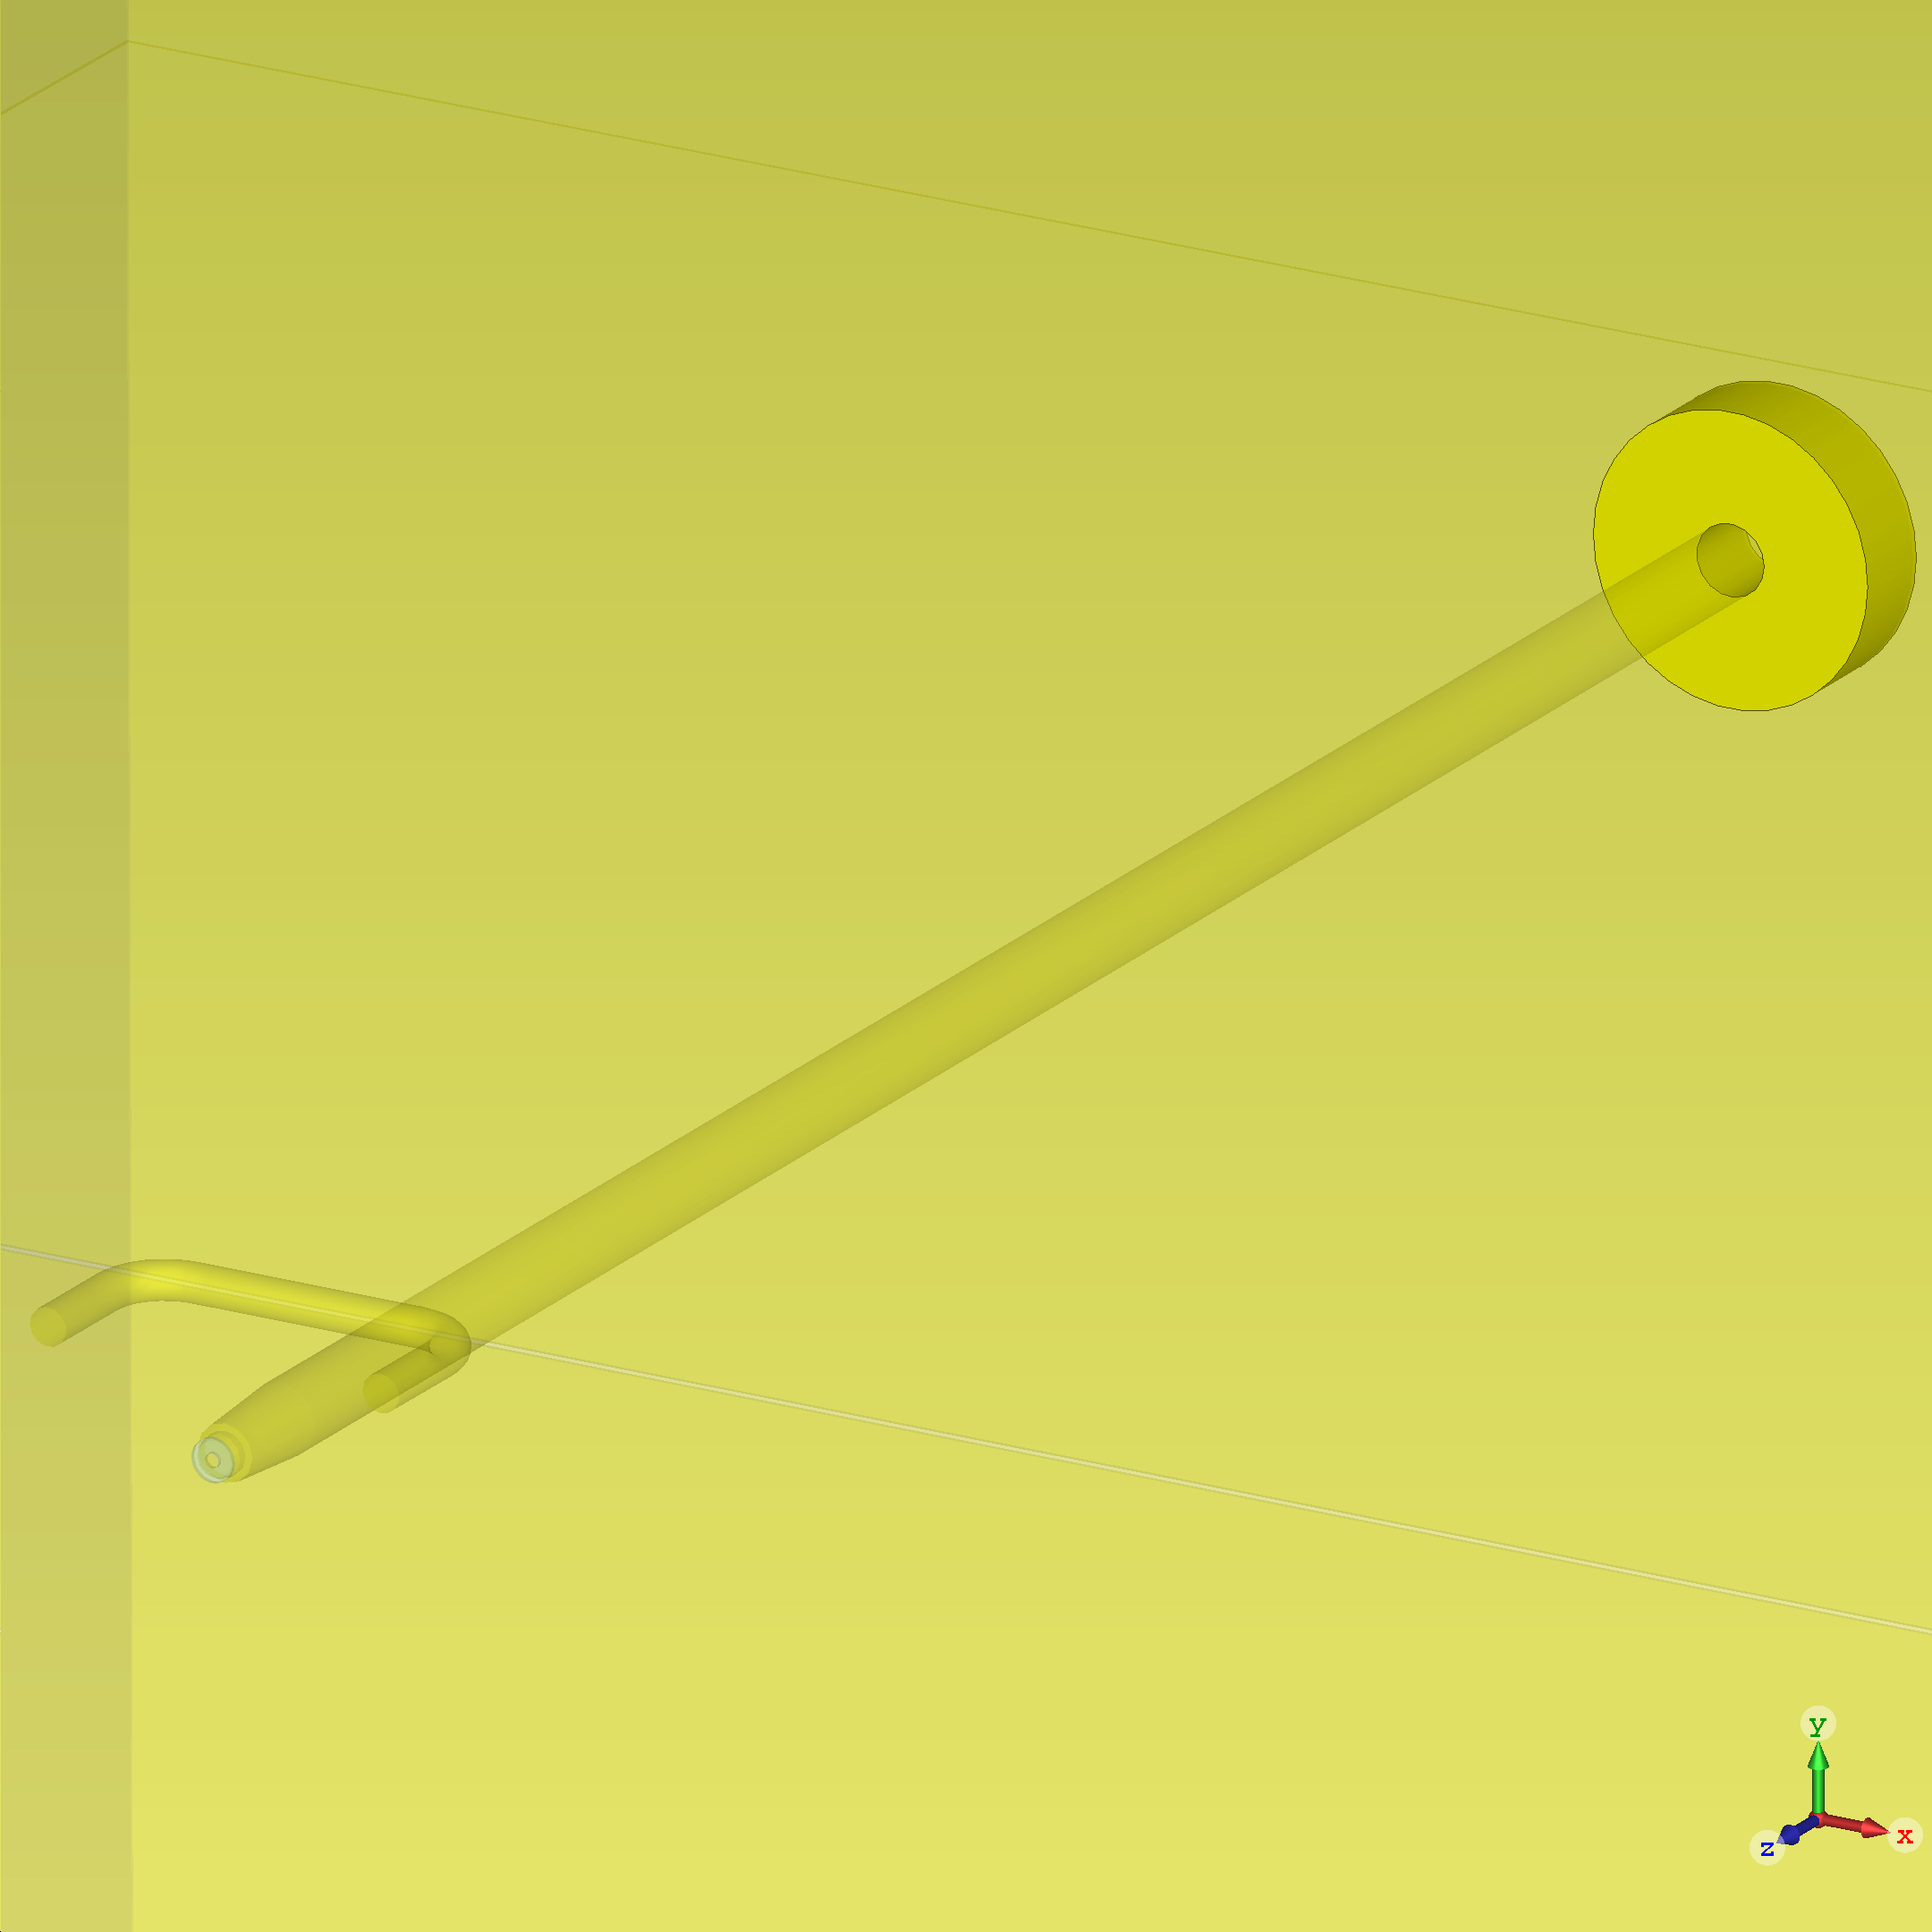
\includegraphics[height=0.3\textwidth]{./Simulation/Block.png}}
                \hspace{0.01\textwidth}
                \subfloat[Holzkonstruktion]{
                    \label{subfig:HolzKonst}
                    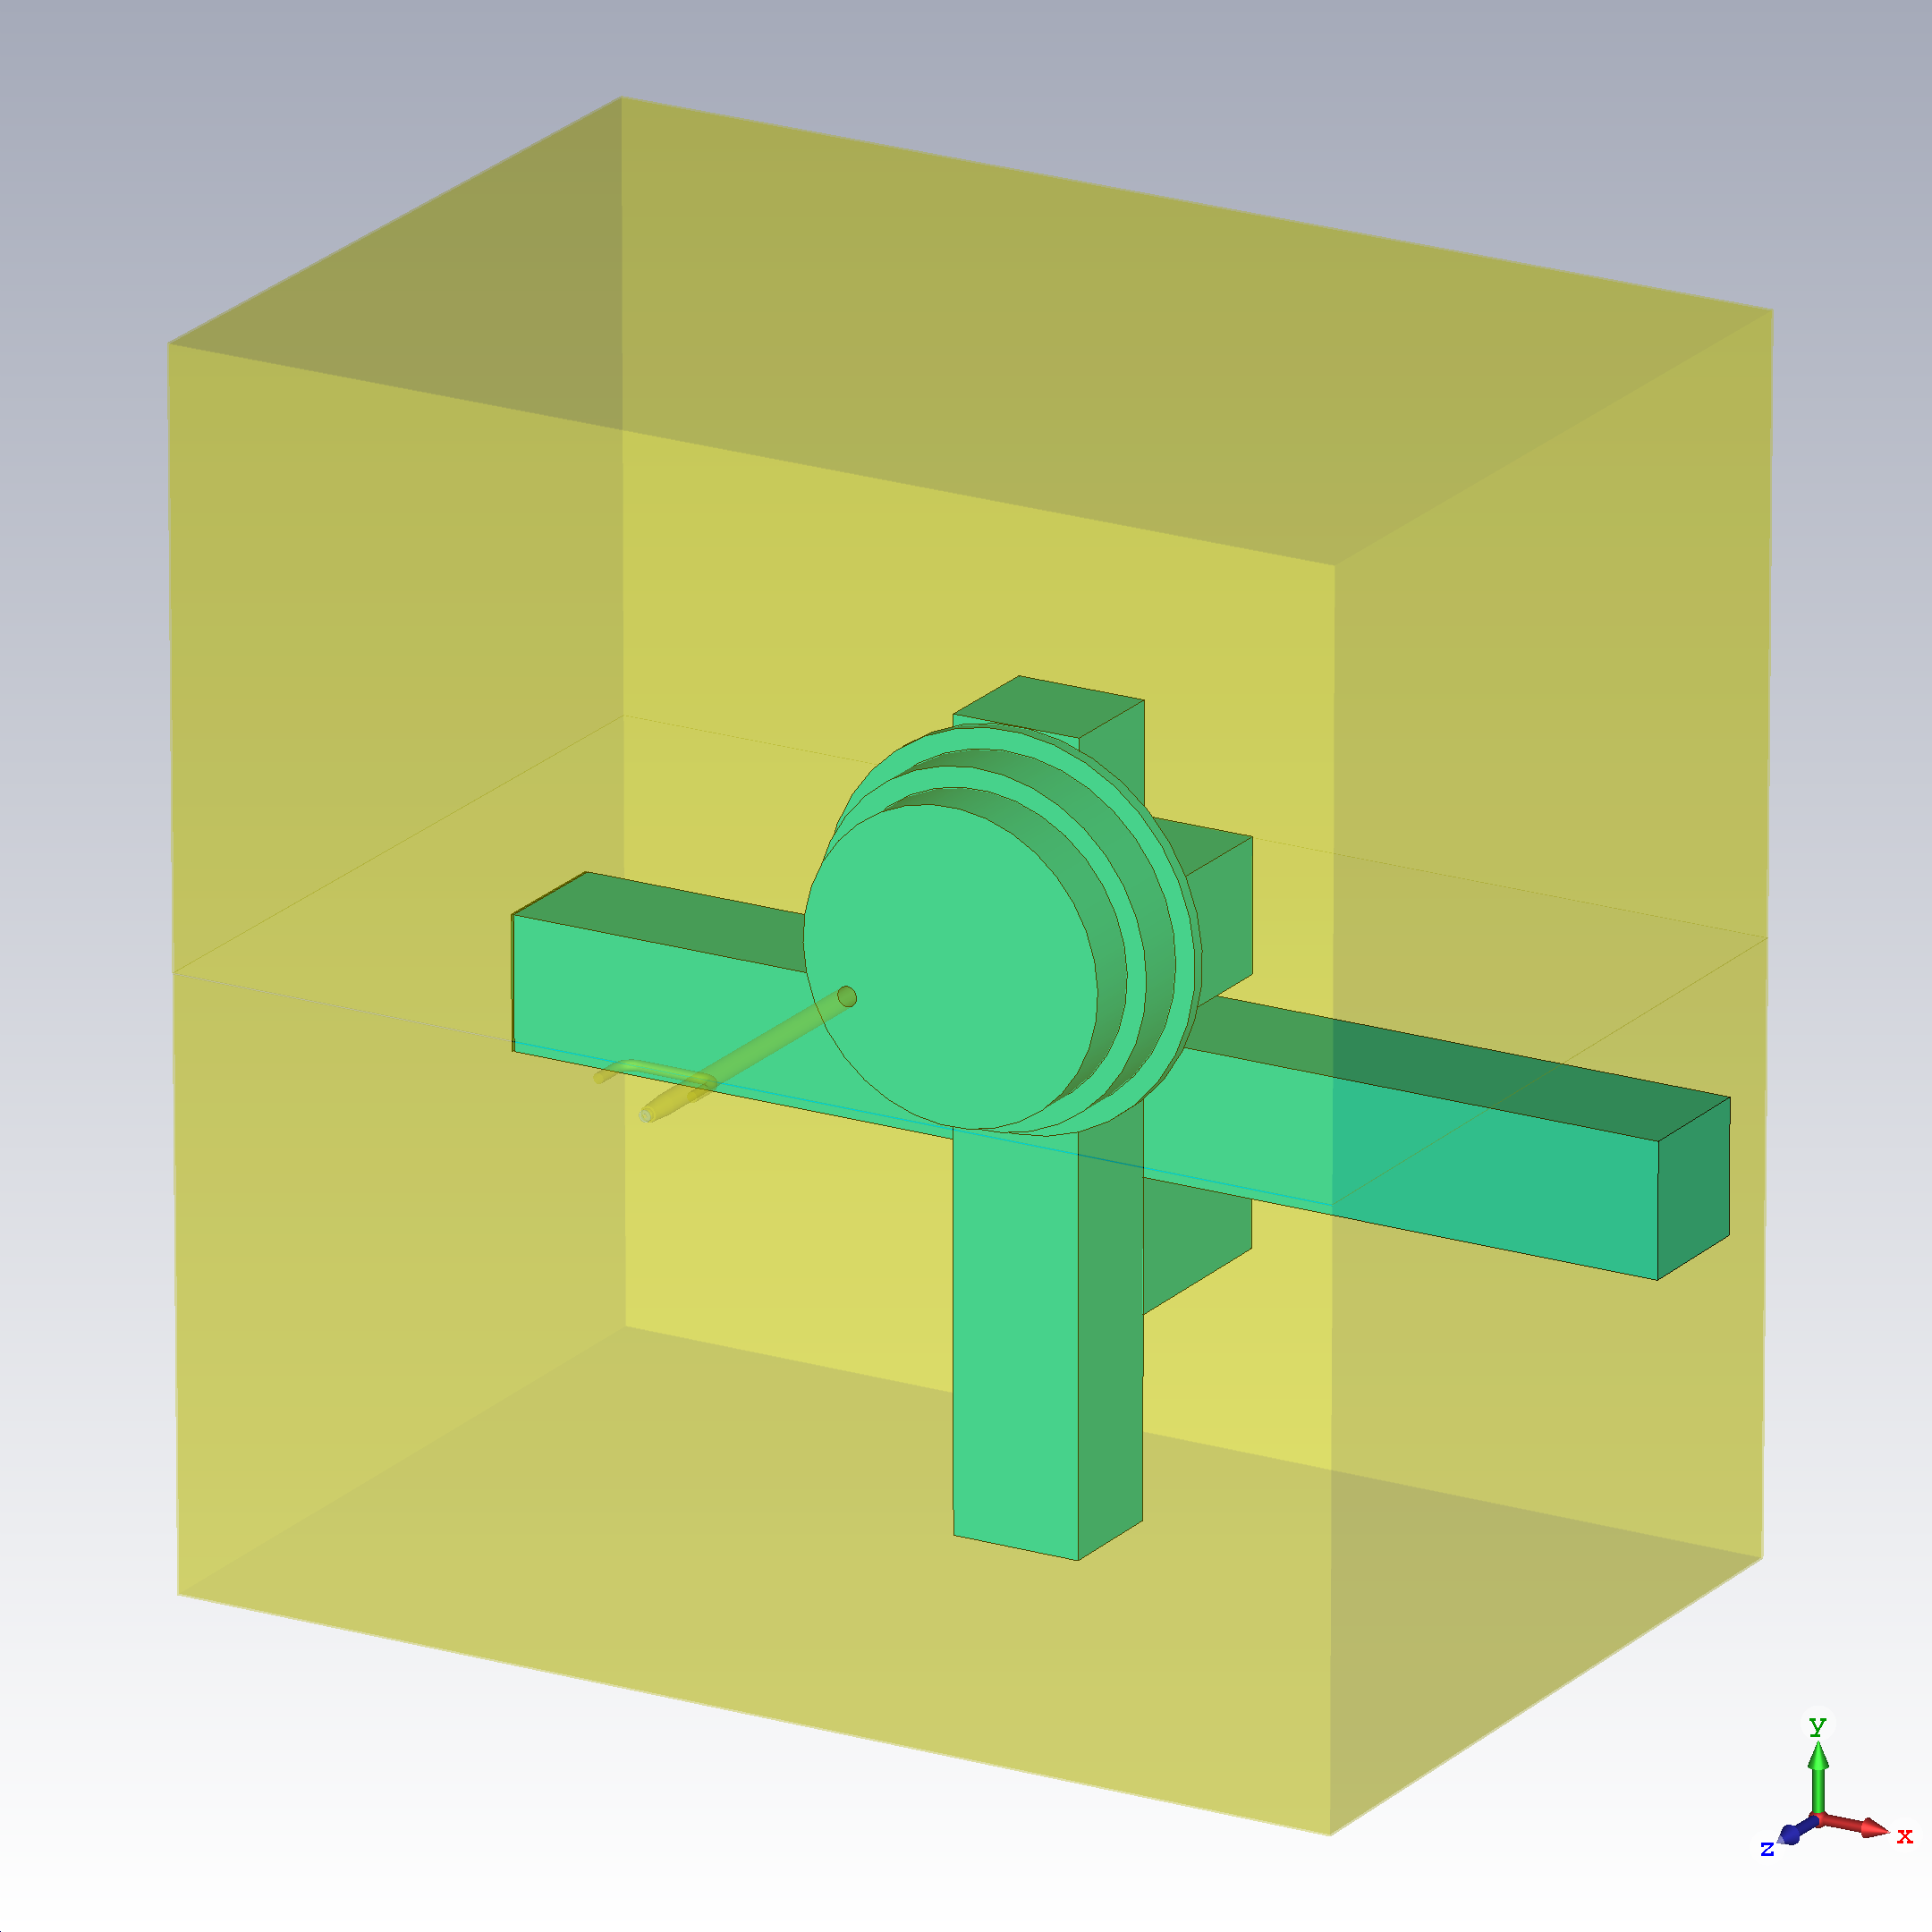
\includegraphics[height=0.3\textwidth]{./Simulation/HolzKonstrukt.png}}
                \caption{Anpassung des Simulationsmodells an den realen Aufbau \protect\subref{subfig:Buegel} Bügel über Einkopplung, \protect\subref{subfig:Block} Kupferzylinder an der Rückwand und \protect\subref{subfig:HolzKonst} die hölzerne Halterung des Ringkerns.}
                \label{fig:AnpassungCST}
            \end{figure}
        
            \subsubsection{Ringkern}
            \label{sec:ringkern}
            Die echten Ringkerne, wie sie bei der GSI benutzt werden, bestehen nicht nur aus dem MA-Material, sondern besitzen einen Innenkreis aus Eisen, der zur Montage dient. Da das Eisen andere magnetische Eigenschaften als das MA-Material besitzt, wurde dies in das Modell übernommen. Die neue Modellierung des Ringkerns mit innerem Eisenring ist in Abbildung~\ref{fig:RKFeRingCST} dargestellt.
                
                \begin{figure}[htb]
                    \centering
                    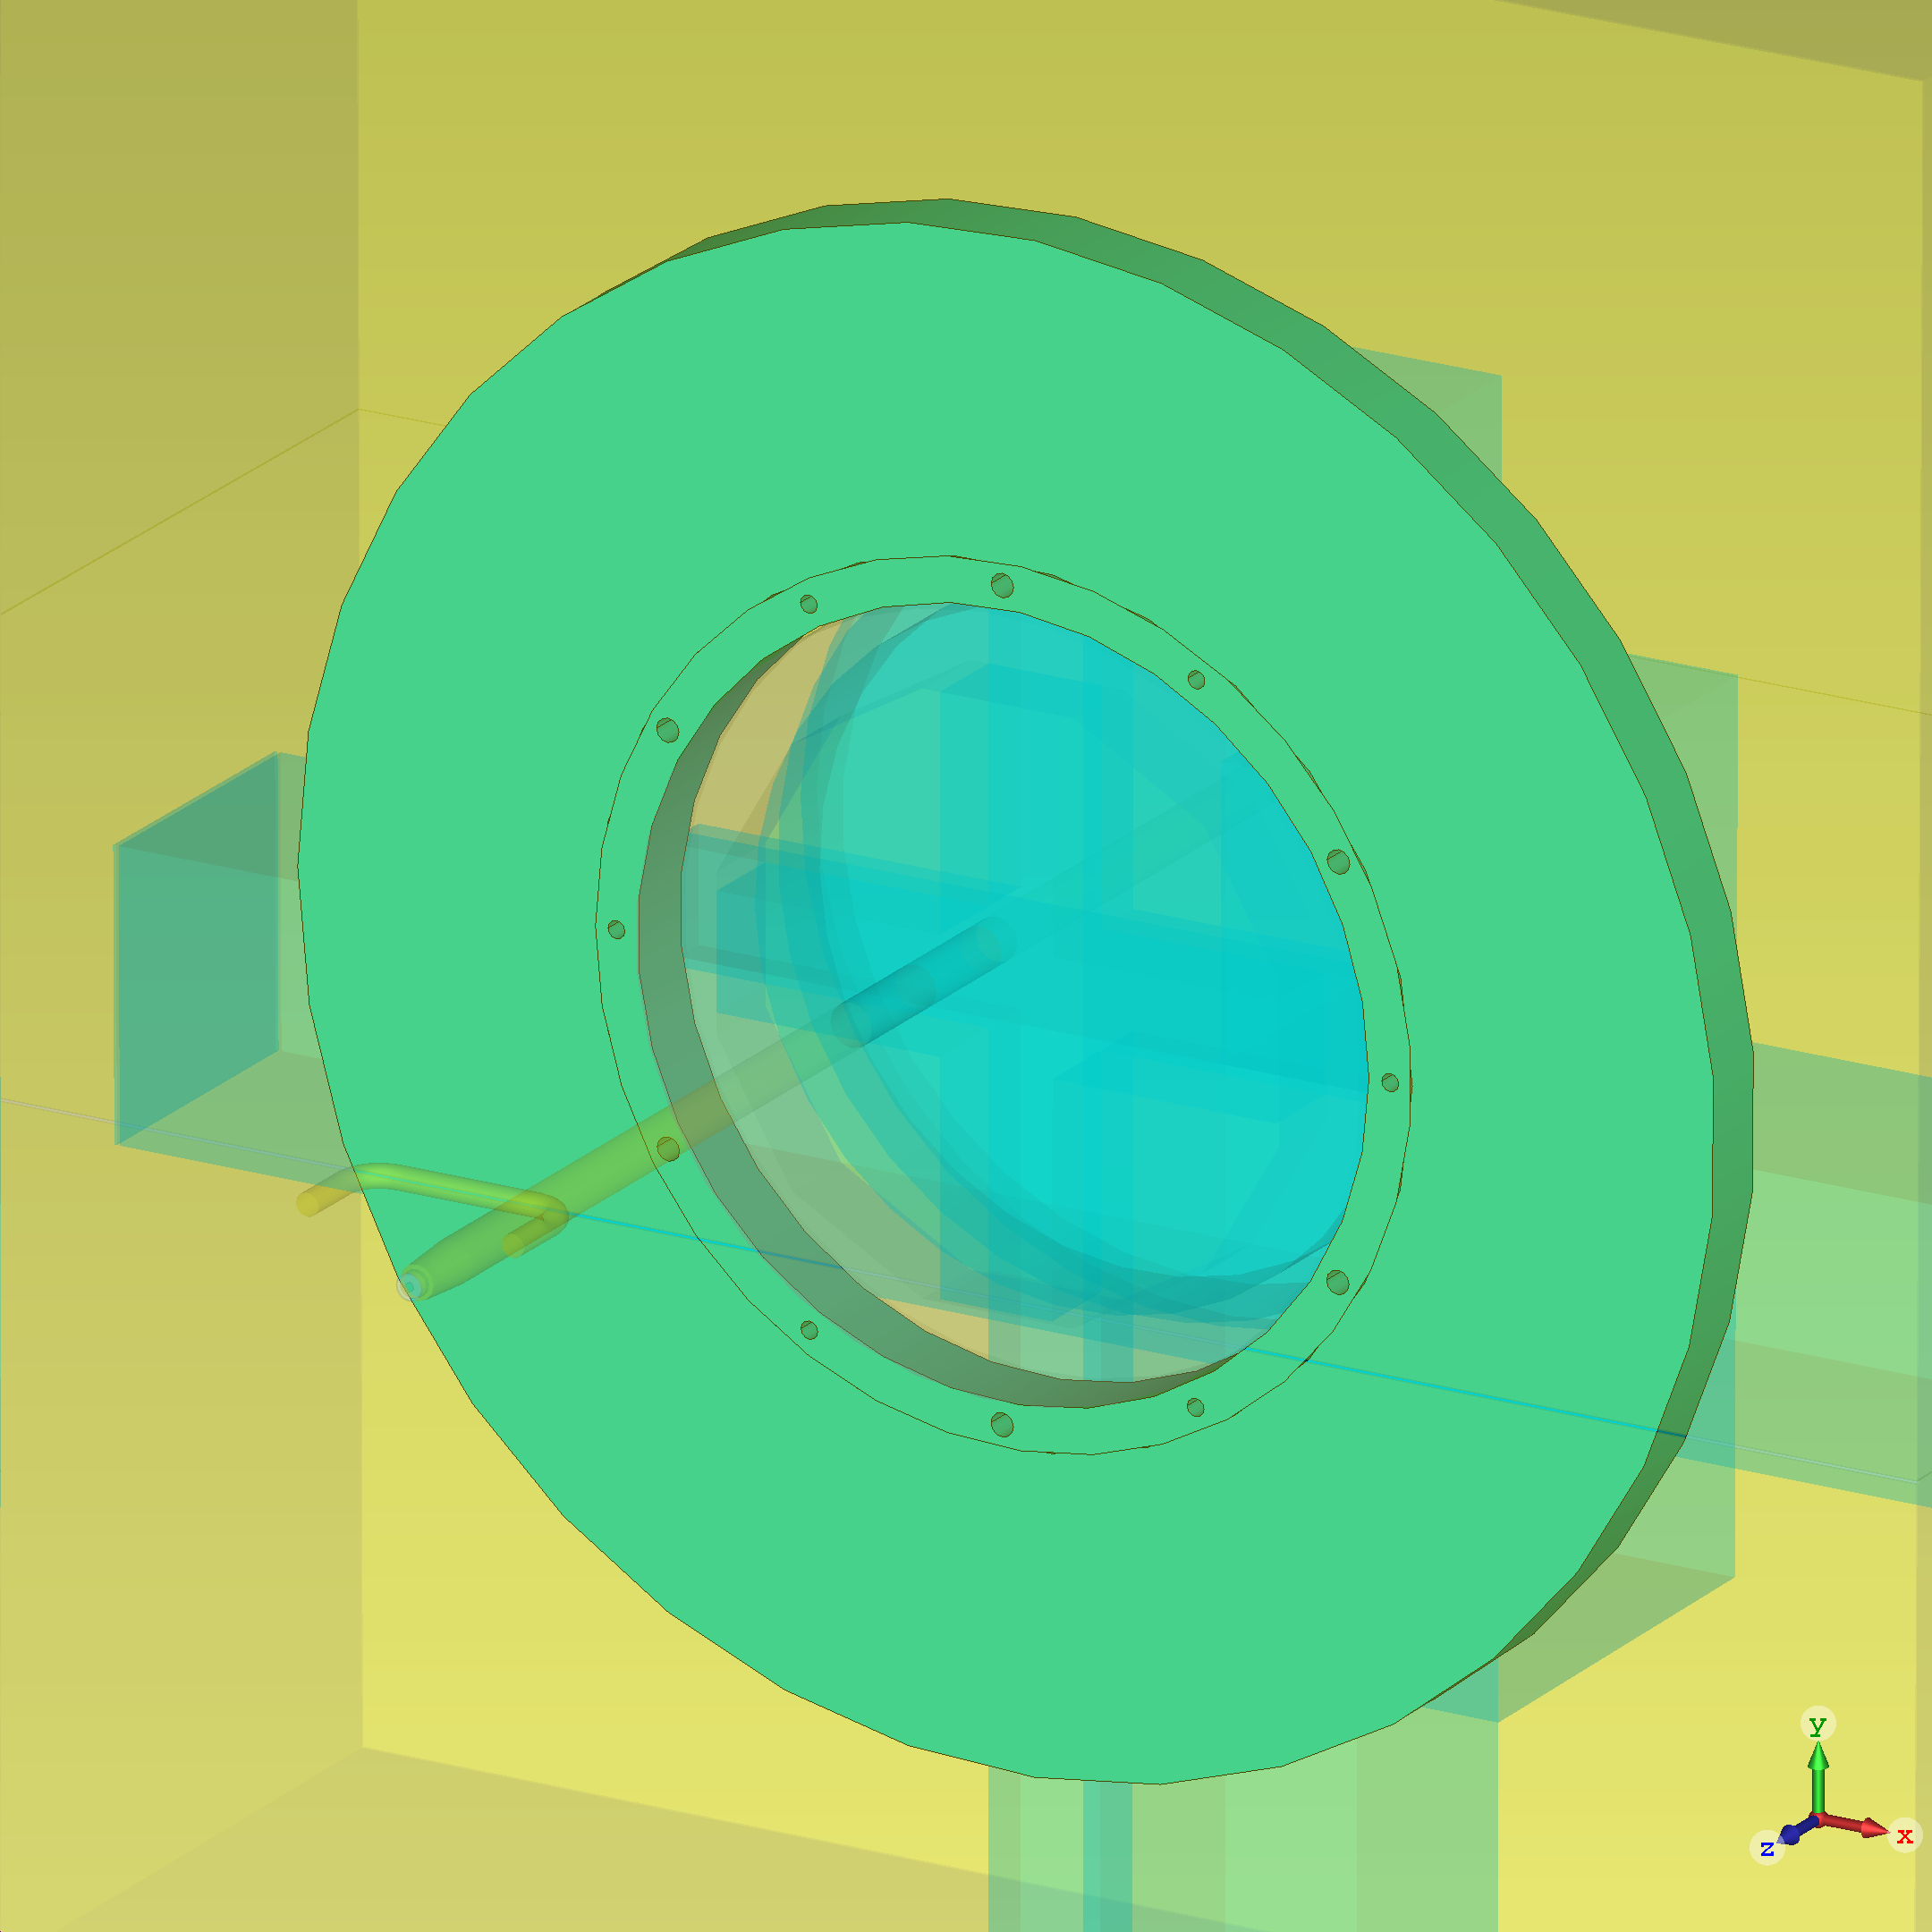
\includegraphics[height=0.4\textwidth]{./Simulation/RKFeRing.png}
                    \caption{Ringkernmodell mit innerem Eisenring}
                    \label{fig:RKFeRingCST}
                \end{figure}
            
            \par
            Des Weiteren wurde für eine bessere Übereinstimmung von Simulation und Messung die magnetische Permeabilität des Ringkernmaterials den Messungen entsprechend aktualisiert. Die Anpassung der Materialparameter basiert auf der Arbeit von Denys Bast~\citep{bast2017ba} und den theoretischen Grundlagen nach ~\citep{Klingbeil2008}.\\
            Die Testbox und der Ringkern können in ein Ersatzschaltbild überführt und damit der Impedanzverlauf analysiert werden. Das Ersatzschaltbild ist in Abbildung~\ref{fig:BoxRKCircuit} dargestellt, dabei wurde die Vorlage aus \citep{bast2017ba} um einen Widerstand ergänzt, der die Verluste der Anordnung nachbildet und für eine Dämpfung der Impedanzamplitude in Resonanz verantwortlich ist. Damit soll das hochfrequente Verhalten der Ersatzschaltung und der Messung besser in Übereinstimmung gebracht werden.\\
            Die Werte für die elektrischen Komponenten der Ersatzschaltung betragen:
                \begin{align}
                    R_{box} &= 16,46~k\Omega \nonumber\\
                    C_{box} &= 6,55~pF \nonumber\\
                    L_{box} &= 528,55~nH \nonumber
                \end{align}
            Die Impedanz dieser Anordnung bestimmt sich nach
                \begin{equation}\label{eq:Zges}
                    \underline{Z}_{ges} = \frac{R_{box}\cdot(\underline{Z}_{rk}+j\omega L_{box})}{R_{box}+(\underline{Z}_{rk}+j\omega L_{box})\cdot(1+j\omega R_{box}C_{box})}.
                \end{equation}
            Daraus lässt sich nun die Impedanz des Ringkerns $Z_{rk}$ bestimmen
                \begin{equation}\label{eq:Zrk}
                \underline{Z}_{rk} = \frac{\underline{Z}_{ges}\cdot(R_{box}+j\omega L_{box}-\omega^2\cdot R_{box}L_{box}C_{box}) - j\omega R_{box}L_{box}}{R_{box}-\underline{Z}_{ges}\cdot(1+j\omega R_{box}C_{box})}.
                \end{equation}
            Wird für $\underline{Z}_{ges}$ die Impedanz aus der Messung eingesetzt, kann die Ringkernimpedanz dieser Messung bestimmt werden.\\
            Nach~\citep{Klingbeil2008} kann diese als Reihenschaltung eines Widerstands $R_{rk}$ und einer Induktivität $L_{rk}$ als $\underline{Z}_{rk} = R_{rk}+j\omega L_{rk}$ betrachtet werden. Für das dissipative $\underline{\mu}_r = \mu' -j\mu''$  des Ringkerns wird in \citep{bast2017ba} angeführt, wie sich mittels der Ersatzschaltung $\mu'$ und $\mu''$ berechnen lassen:
                \begin{equation}
                    \mu' = \frac{L_{rk}\cdot 2\pi}{d\cdot ln\frac{r_a}{r_i}}
                \end{equation} 
                \begin{equation}
                \mu'' = \frac{R_{rk}\cdot\mu'}{\omega\cdot L_{rk}} .
                \end{equation}
            
                \begin{figure}[htb]
                    \centering
                    \begin{tikzpicture}
                    \node[above] at (-0.25,1.6) {$Z_{ges}$};
                    \draw (-0.5,1.4) -- (0.1,1.4);
                    \draw (-0.5,1.6) -- (0.1,1.6);
                    \path[fill=black, draw=black]
                        (0.1,1.3)  -- (0.1,1.7)  -- (0.5,1.5) --  (0.1,1.3);
                    \begin{circuitikz}
                    \draw
                    (2,0) to [resistor =$R_{box}$] (2,3)
                    (5,0) to [C, l=$C_{box}$] (5,3)
                    (5,3) to [L, l=$L_{box}$] (9,3)
                    (9,3) to [short, *-] (10,3)
                    (9,0) to [short, *-] (10,0)
                    (10,3) to [resistor =$Z_{rk}$] (10,0)
                    (0,3) to [short, *-] (5,3)
                    (0,0) to [short, *-] (5,0)
                    (8,3) to [short, -*] (9,3)
                    (5,0) to [short, -*] (9,0);
                    % 		(0,0) to [short, *- , i_=$I_5$] (1.5,-2);
                    \end{circuitikz}
                    \end{tikzpicture}
                    \caption{RLC-Ersatzschaltbild f\"ur die Testbox Modellierung mit Eingebrachtem Ringkern als Last.}
                    \label{fig:BoxRKCircuit}
                \end{figure}
                
            Ausgehend vom angepassten, dissipativen $\underline{\mu}_r$ kann nun die Simulation aktualisiert werden. Dazu werden die bestimmten Werte für $\mu'$ und $\mu''$ als Materialparameter in CST hinterlegt.
           
        \subsection{Erweiterung des Modells}
        Wie bereits in Kapitel~\ref{chap:messaufbau} erläutert, wurde die Testbox für die einfachere Montage der Kurzschlüsse und die erhöhte Reproduzierbarkeit der Messungen modifiziert und um ein kreuzförmiges Gestell aus Holz, sowie einen nichtleitenden Ring mit einem Polygonzug als Innenkreis erweitert (Geometrie und Beschreibung siehe Kapitel~\ref{chap:messaufbau}). Diese Modifikationen sind mit CST geometrisch genau nachgebildet (siehe Abb.~\ref{fig:KreuzPolygonCST}). Für das Holzkreuz wurden die selben Materialparameter verwendet, die für die Holzkreise hinterlegt sind, da es sich auch hierbei das Pressspanholz handelt.
        
            \begin{figure}[htb]
                \centering
                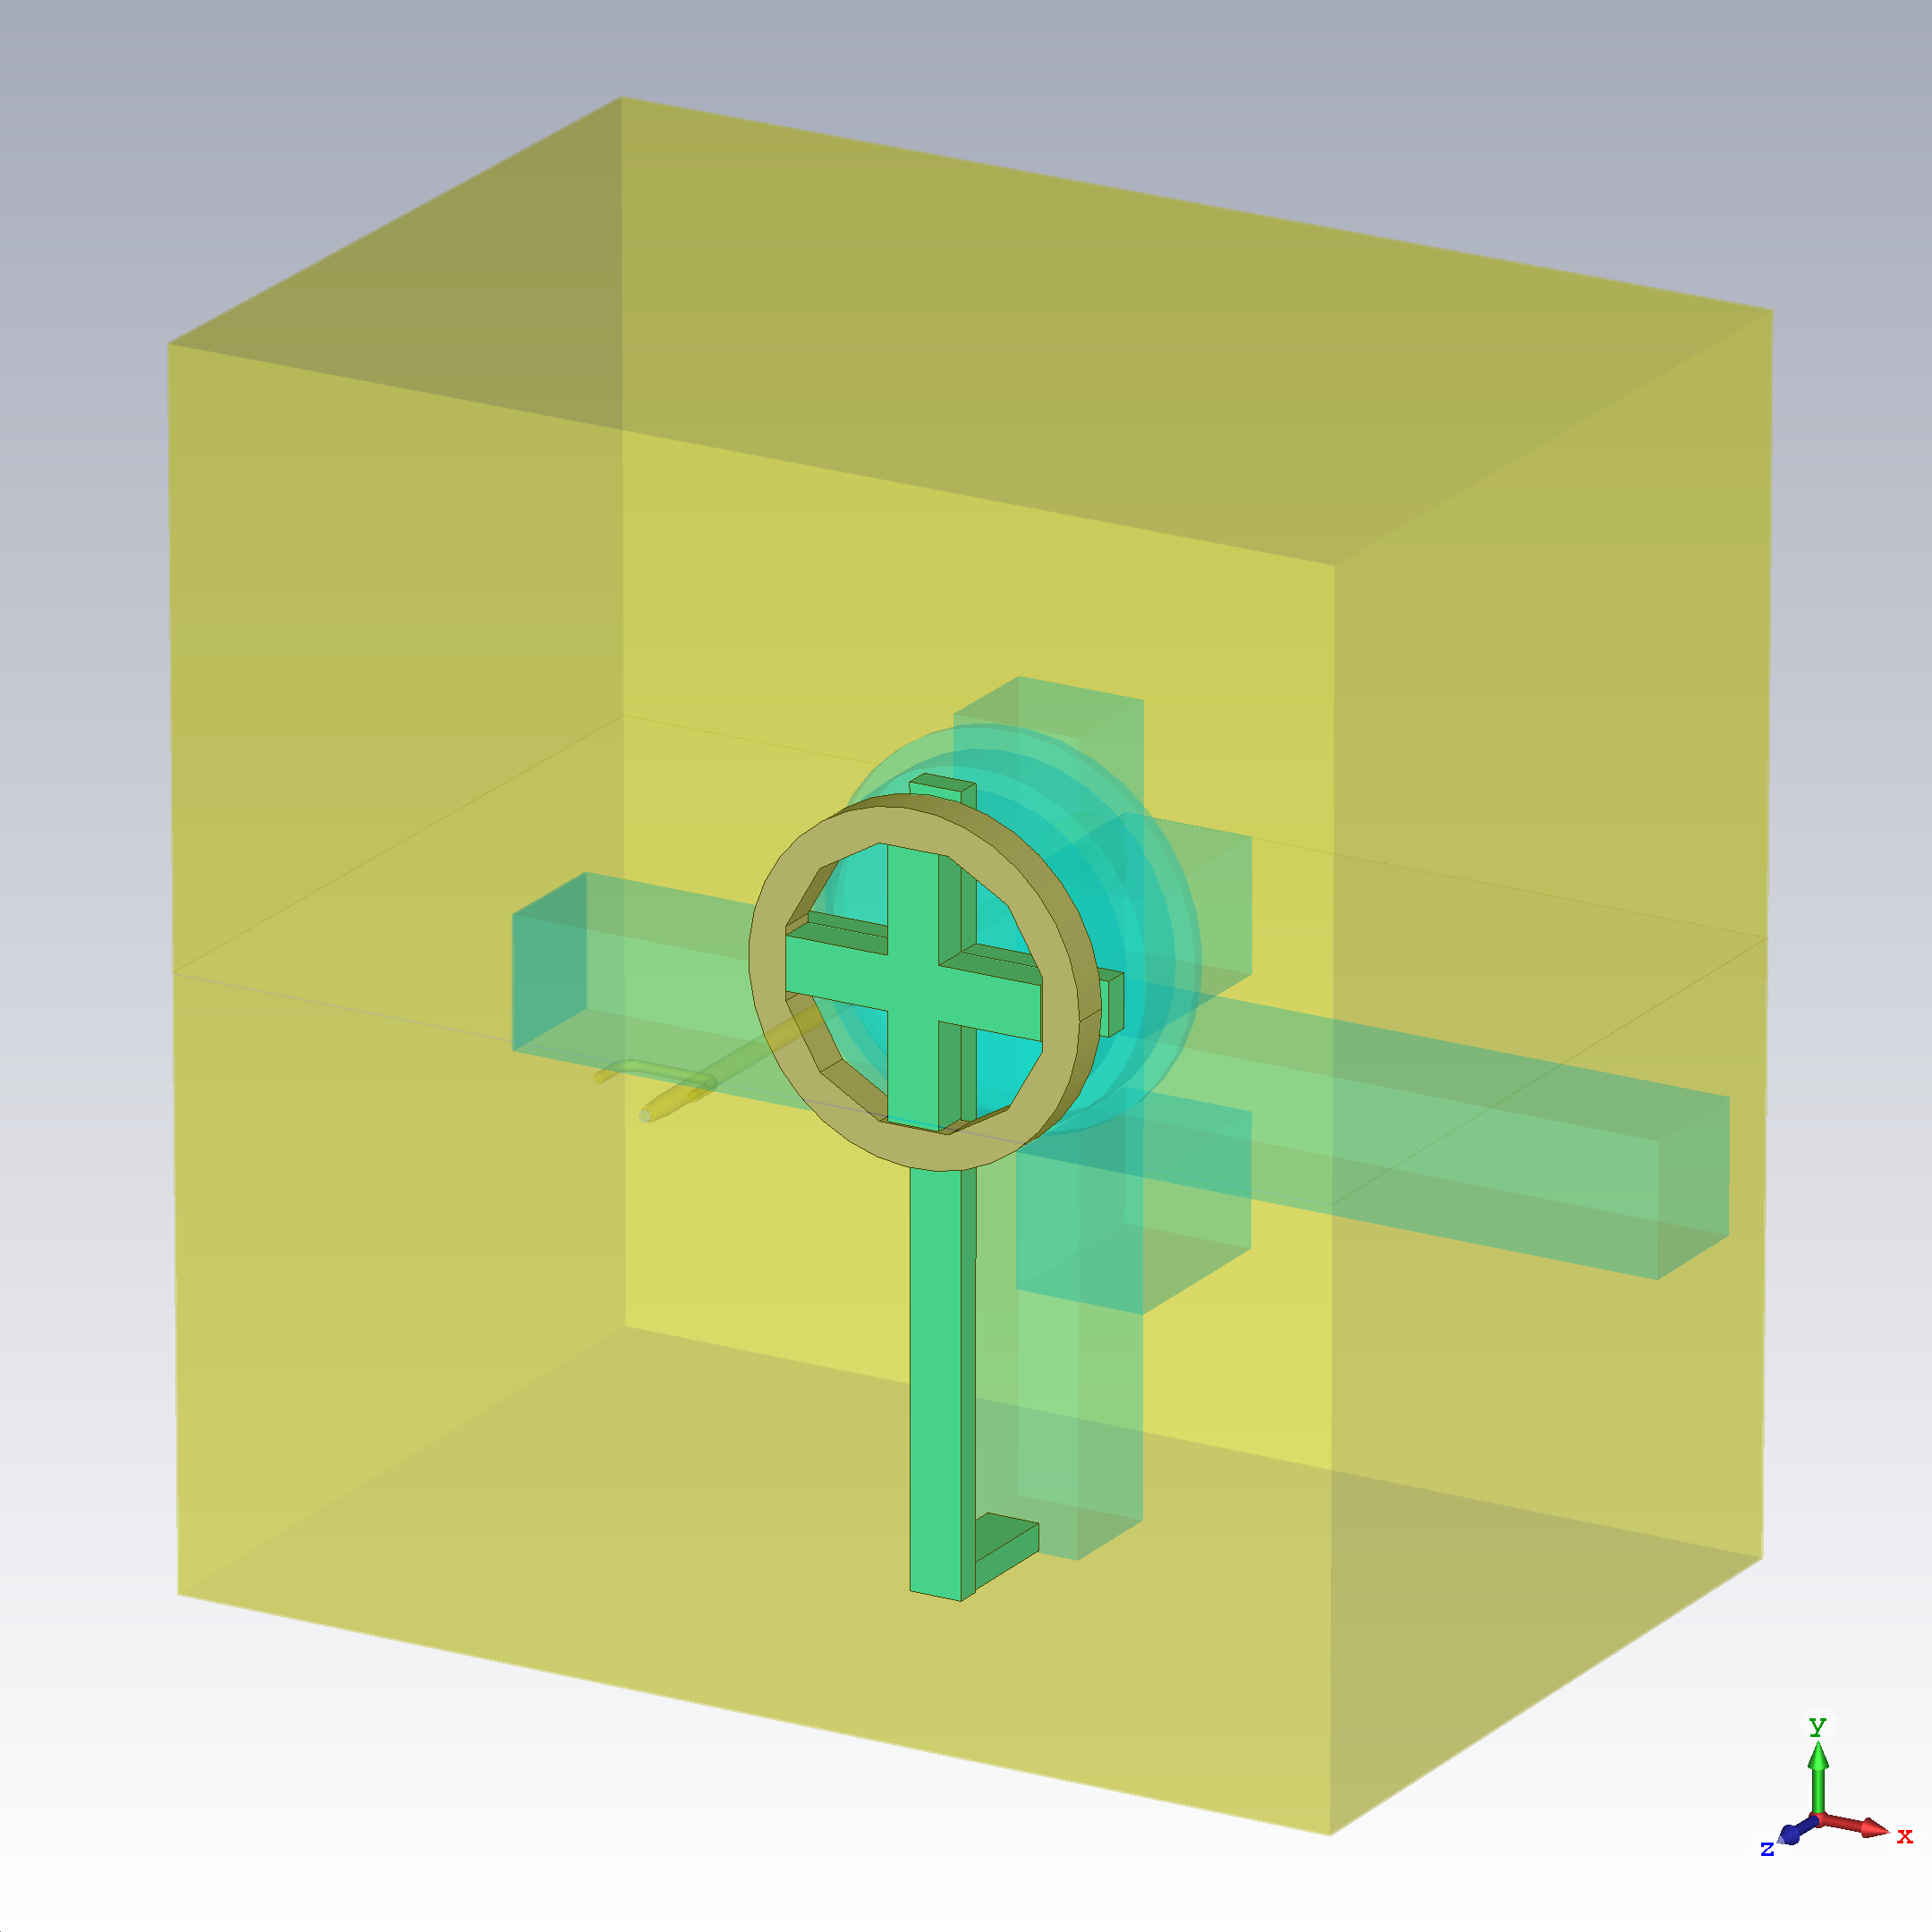
\includegraphics[height=0.4\textwidth]{./Simulation/KreuzPolygon.png}
                \caption{Erweiterung der Testbox um die Holzkreuzhalterung und den Polygonzug zur Befestigung der Kurzschlüsse}
                \label{fig:KreuzPolygonCST}
            \end{figure}
        
    \section{Durchführung}
        \subsection{Einstellungen in CST und Wahl des Numerischen Lösers}
        Die Simulation in CST wurde weitgehend mit den Einstellungen und dem Löser durchgeführt, wie sie in \citep{bast2017ba} beschrieben werden. Einige wichtige Punkte werden an dieser Stelle kurz aufgegriffen, um ein Wiederholen der Simulationen zu ermöglichen.
        \par
        Die Modelle wurden mit dem Frequency Domain Solver von CST simuliert, der die Maxwell Gleichungen im Frequenzbereich numerisch behandelt, da es sich bei der Testbox um ein resonantes Konstrukt handelt und es sich bei den betrachteten Messdaten (Impedanzverläufe) um elektrische Parameter im Frequenzbereich handelt.\\
        Die räumliche Diskretisierung der Modelle erfolgt mit einer adaptiven Gitterverfeinerung von Tetraedern und Curved-Elements, die besonders für die Approximation gekrümmter Strukturen geeignet sind.\\
        Der betrachtete Frequenzbereich der Simulation wurde $\SI{0,01}{\mega\hertz}$ bis $\SI{100}{\mega\hertz}$ gewählt, da der Frequqenzbereich in dem die Ringkerne betrieben werden niedriger ist und dies der für den Impedanzverlauf der Testbox relevante Bereich ist, weil die Resonanz zwischen $\SI{80}{\mega\hertz}$ bis $\SI{90}{\mega\hertz}$ liegt.\\
        Der numerische Löser ist mit einer Ordnung von 2 gewählt und die Genauigkeit für die Lösung der Gleichungssysteme auf $10^{-4}$ eingestellt.
        \par 
        Im Anschluss an die numerische Berechnung der elektromagnetischen Felder im Frequenzbereich wird in einem Post-Processing-Schritt die Eingangsimpedanz des Modells aus dem Streuparameter $S_{11}$ berechnet
            \begin{equation}
                Z = Z_0 \cdot\frac{1+S_{11}}{1-S_{11}},
            \end{equation}
        mit $Z_0 = \SI{50}{\Omega}$.
        
        \subsection{Variation der Kurzschlussparameter}
        Für die Gegenüberstellung und Vergleichbarkeit von Simulation und Messung werden die Kurzschlüsse mit den gleichen Variationen der zu untersuchenden Parameter (siehe Kapitel~\ref{chap:messaufbau}) und der Messung entsprechenden Anordnung am Ringkern  nachgebildet.\\
        Die Bilder der verschiedenen Anordnungen und Kurzschlussausführungen sind in Kapitel~\ref{chap:ergebnis} zu finden. In Abbildung~\ref{fig:ringcorenumberCST} ist dabei die Variation in der Anzahl der Kurzschlüsse dargestellt, die um den Ringkern angebracht sind. Abbildung~\ref{fig:ringcorewidthCST} zeigt die Simulation der verschiedenen Breiten und in Abbildung~\ref{fig:ringcoreheightCST} sind die verschiedenen Ringkernlängen zu sehen. Für die Simulation und Messung der Breiten-, Längen- und Dickenvariation wurde immer die in den Abbildungen gezeigte Position für einen Kurzschluss gewählt, der zweite Kurzschluss wurde dem ersten gegenüber angebracht.

